\documentclass[12pt,a4paper,twoside,openright,headsepline,footsepline]{scrreprt}

\usepackage[top=1.5cm,bottom=1.5cm,footskip=.8cm,footnotesep=1cm,includeheadfoot]{geometry}

\usepackage[ngerman]{babel}

\usepackage[utf8]{inputenc}

\usepackage{scrpage2}
\pagestyle{useheadings}

\usepackage[pdftex]{graphicx}
\usepackage{epstopdf}


\usepackage{cite}

\usepackage{amsmath}
\usepackage{amssymb}

\usepackage{amsthm}
\theoremstyle{definition}
\newtheorem*{ziel}{Zielsetzung}
\newtheorem{defi}{Definition}[section]
\newtheorem*{fazit}{Fazit}

\usepackage{dsfont}
\newcommand{\R}{\mathds{R}}
\renewcommand{\d}{\mathrm{d}}

\usepackage{siunitx}

\sloppy


\usepackage{hyperref}


\begin{document}
\begin{frontmatter}
  \title{Curvature approximation on surfaces -- A Discrete Exterior Calculus Approach}

  \author{I.~Nitschke\fnref{fn1}}
  \ead{ingo.nitschke@tu-dresden.de}
  
  \author{A.~Voigt\fnref{fn1,fn2}}
  \ead{axel.voigt@tu-dresden.de}

  \fntext[fn1]{Department of Mathematics, TU Dresden, 01062 Dresden, Germany}
  \fntext[fn2]{Center of Advanced Modeling and Simulation, TU Dresden, 01062 Dresden, Germany}

  \begin{abstract}
    Lorem ipsum dolor sit amet, consetetur sadipscing elitr, sed diam nonumy eirmod tempor invidunt ut labore et dolore magna aliquyam erat, sed diam voluptua. At vero eos et accusam et justo duo dolores et ea rebum. Stet clita kasd gubergren, no sea takimata sanctus est Lorem ipsum dolor sit amet. Lorem ipsum dolor sit amet, consetetur sadipscing elitr, sed diam nonumy eirmod tempor invidunt ut labore et dolore magna aliquyam erat, sed diam voluptua. At vero eos et accusam et justo duo dolores et ea rebum. Stet clita kasd gubergren, no sea takimata sanctus est Lorem ipsum dolor sit amet. Lorem ipsum dolor sit amet, consetetur sadipscing elitr, sed diam nonumy eirmod tempor invidunt ut labore et dolore magna aliquyam erat, sed diam voluptua. At vero eos et accusam et justo duo dolores et ea rebum. Stet clita kasd gubergren, no sea takimata sanctus est Lorem ipsum dolor sit amet.
  \end{abstract}

  \begin{keyword}
    Surfaces \sep Curvature \sep DEC
  \end{keyword}
\end{frontmatter}

\section{Introduction}
Lorem ipsum dolor sit amet, consetetur sadipscing elitr, sed diam nonumy eirmod tempor invidunt ut labore et dolore magna aliquyam erat, sed diam voluptua. At vero eos et accusam et justo duo dolores et ea rebum. Stet clita kasd gubergren, no sea takimata sanctus est Lorem ipsum dolor sit amet. Lorem ipsum dolor sit amet, consetetur sadipscing elitr, sed diam nonumy eirmod tempor invidunt ut labore et dolore magna aliquyam erat, sed diam voluptua. At vero eos et accusam et justo duo dolores et ea rebum. Stet clita kasd gubergren, no sea takimata sanctus est Lorem ipsum dolor sit amet. Lorem ipsum dolor sit amet, consetetur sadipscing elitr, sed diam nonumy eirmod tempor invidunt ut labore et dolore magna aliquyam erat, sed diam voluptua. At vero eos et accusam et justo duo dolores et ea rebum. Stet clita kasd gubergren, no sea takimata sanctus est Lorem ipsum dolor sit amet.

  
  \begin{figure}
    \centering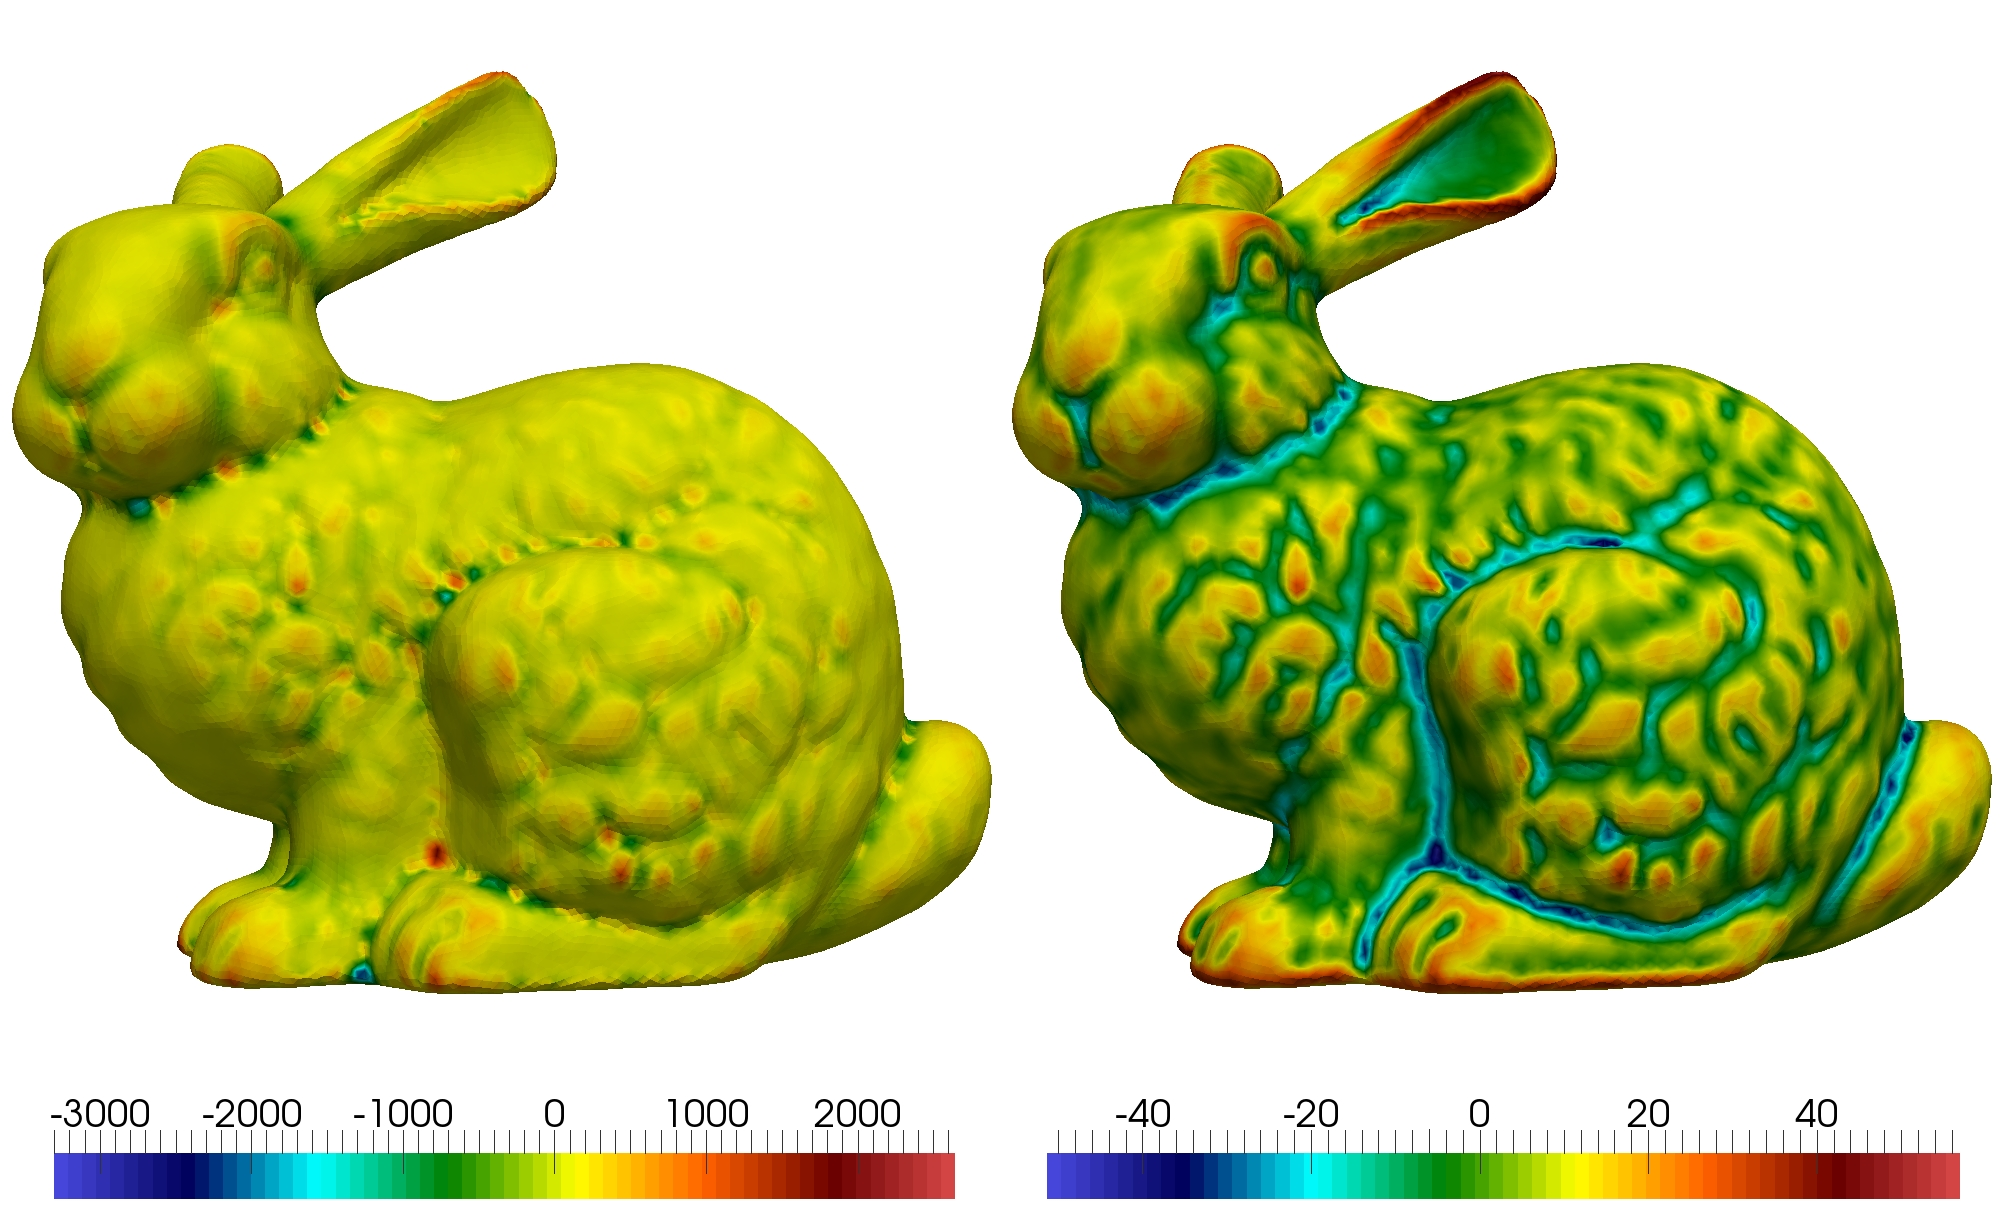
\includegraphics[width=.45\textwidth]{bilder/bunnyCurvature.jpg}
    \centering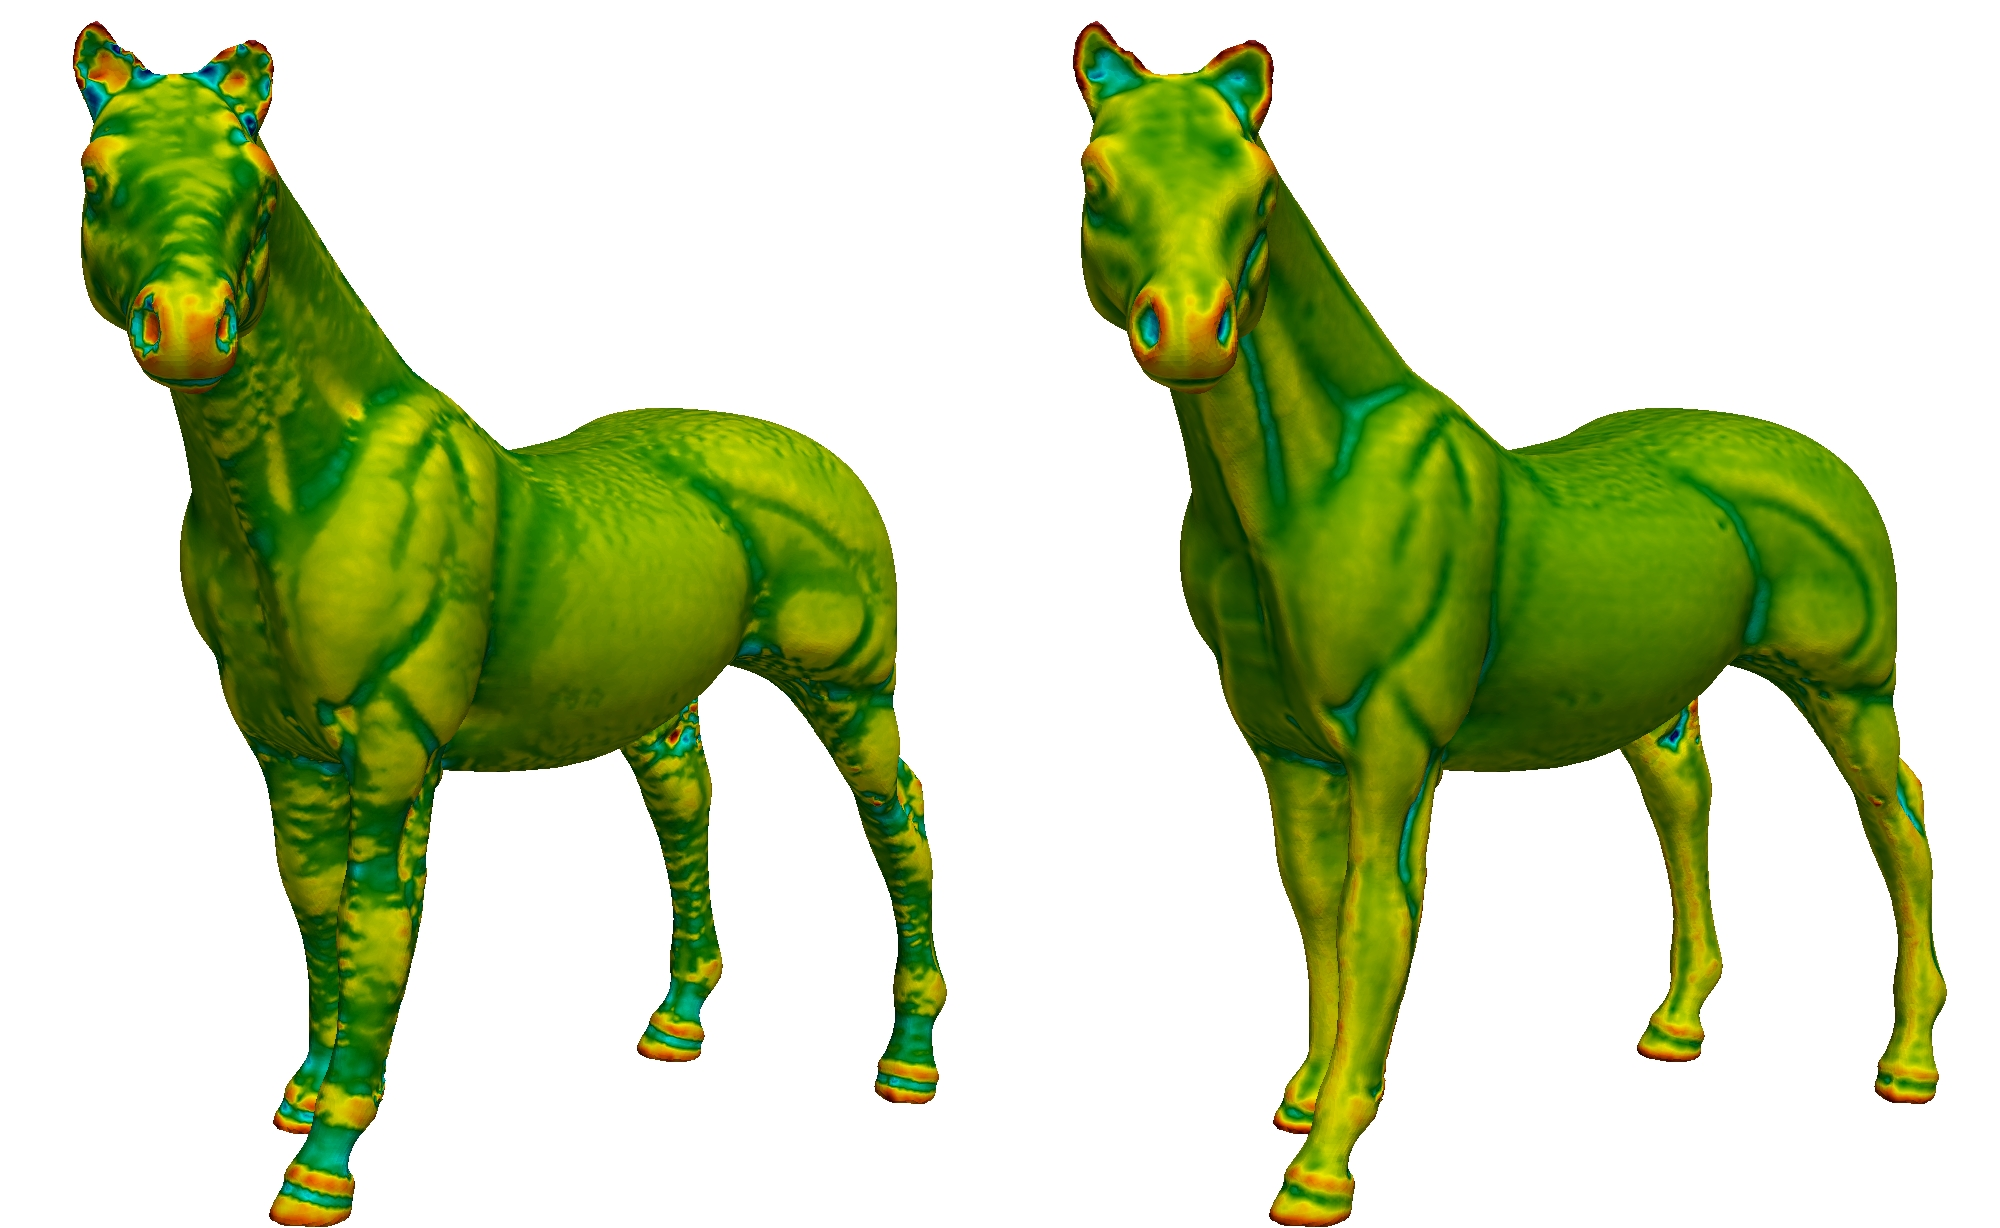
\includegraphics[width=.45\textwidth]{bilder/horseCurvature.jpg}
    \centering
\includegraphics[width=.45\textwidth]{bilder/colourBar.jpg}
    \caption{Surface curvature approximations of the Stanford Bunny and a horse.
             Left: Gaussian curvature \( K \) (square root scaled colours).
             Right: Mean curvature \( H \) (linear scaled colours)}
    \label{figBunnyHorseCurvature}
  \end{figure}


\section{Discrete Exterior Calculus (DEC)}
  The Discrete Exterior Calculus \citep{hirani, desbrun} defines discrete differential \mh{p}{forms} on a triangulated mesh (simplicial complex).
  For surface meshes, i.e. triangulated orientable \mh{2}{manifolds}, the degree of the discrete \mh{p}{forms} is 0, 1 or 2
  and their are represented by scalars on vertices, edges, triangles or chains of them. 
  Operators for the differential forms, like the exterior derivation \( \exd \) or the hodge star \( \star \), can be approximated by expressions on the discrete
  geometrical structure. 
  E.g. the integral over a triangle of the exterior derivation \( \exd \) for a \mh{1}{form} can be expressed as the integral of this
  \mh{1}{form} over the boundaries edges of the triangle. 
  This follows directly from the Stokes Theorem \citep[Ch. 7]{marsden}. 
 
  \subsection{Discrete manifolds}
    In our setting, the surface meshes are linear triangulations of orientable closed \mh{2}{manifolds}.
    Such a Triangulation are sets of \mh{p}{simplices} \( \left\{ \sigma^{p} \right\} \) of the same degree \( p \), e.g. sets of vertices,
    edges and triangles, and form a simplicial complex of dimension \( n=2 \).
    A simplicial complex \( K \) comply two essential rules:
    \begin{enumerate}
      \item Every face of a simplex \( \sigma^{p}\in K \) is in \( K \).
      \item The intersection of two simplices in \( K \) is either in \( K \) or empty.
    \end{enumerate}
    We shortly write \( \sigma^{q}\prec\sigma^{p} \) (or \( \sigma^{p}\succ\sigma^{q}) \)), 
    iff \( q<p \) and \( \sigma^{q} \) is a face of \( \sigma^{p} \). 
    It is required, that the polytop
    \begin{align}
      |K| &:= \bigcup_{\sigma\in K} \sigma 
    \end{align}
    of \( K \) is a \mh{C^{0}}{manifold} and we call \( K \) a manifold-like simplicial complex.
    For a higher consistence to the smooth model, we assume that the simplicial complex is orientable,
    i.e. all triangles \( \sigma^{2}\in K \) have the same orientation.
    The orientation of a triangle is define as one of the two equivalence classes, that arise from the kind of counting the vertices
    (clockwise or counterclockwise).
    We write \( \sigma^{2}=\left[ v_{0}, v_{1}, v_{2} \right] \) to mark the order of the vertices \( v_{i} \).
    In the same manner a edge \( \sigma^{1} = \left[ v_{0}, v_{1} \right] \) get an declared orientation.
    Such a manifold-like orientable simplicial complex is called a primal mesh.

    For the existence of a dual mesh, we also need, that the primal mesh is well-centered, 
    i.e. for all triangles \( \sigma^{2}\in K \) the circumcenter \( c(\sigma^{2}) \) lies in the interior of \( \sigma^{2} \).
    A dual mesh \( \csd K \) is the circumcenter subdivision of a well-centered primal mesh \( K \).
    For a explanatory example see figure \ref{figExSubdivision}.
    The dual mesh is also a primal mesh, but it is not well-centered.

    \begin{figure}
      \begin{minipage}[htp]{.24\textwidth}
        \centering
        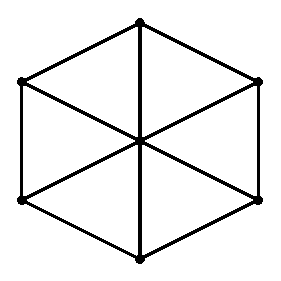
\includegraphics[width=.9\textwidth]{bilder/tikz/K.eps}
      \end{minipage}\hfill
      \begin{minipage}[htp]{.24\textwidth}
        \centering
        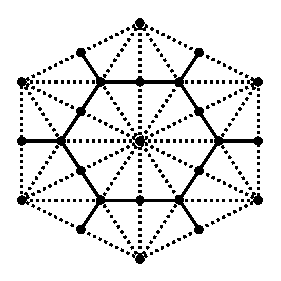
\includegraphics[width=.9\textwidth]{bilder/tikz/CsdK.eps}
      \end{minipage}
      \caption{Example of a circumcenter subdivision.
               Left: A primal mesh \( K \).
               Right: The resultant dual mesh \( \csd K \). 
               All new vertices are the circumcenters of the triangles and edges.
               The solid lines highlights the edges of the Voronoi mesh \( \star K \leq \csd K \).}
      \label{figExSubdivision}
    \end{figure}

    \subsection{Chains}
    An important role in the DEC are chains. 
    A \mh{p}{chain} is the formal sum of \mh{p}{simplices} with coefficients in \( \Z \). 
    Therewith, we denote the space of all \mh{p}{chains} of \( K \)  by
    \begin{align}
      C_{p}(K) &:= \left\{\sum_{\sigma\in K^{(p)}}a_{\sigma}\sigma \middle| a_{\sigma}\in\Z \right\} \formpunkt
    \end{align}
    \( K^{(p)} \) is the set of all \mh{p}{simplices} of \( K \). 
    For chains we can use the universal property, because \( C_{p}(K) \) is a free abelian group with the generating set \( K^{(p)} \).
    Hence, the diagram
    \begin{align}
    \begin{xy}
      \xymatrix{
        C_{p}(K) \ar[rd]^{\widehat{op}} & \\
        K^{(p)} \ar@^{(->}[u] \ar[r]_{op}& \mathfrak{A}
      }
    \end{xy}
  \end{align}
  commutes for a arbitrary abelian group \( \mathfrak{A} \) and homomorphism \( op = \widehat{op}|_{K^{(p)}} \) 
  and \( \widehat{op} \) is unique determinated by \( op \),
  i.e. it is quit enough to define operators for chains only on the simplices. 
  
  \subsection{Geometrical operators}
    The two momentous operators on chains are the boundary operator \( \partial \) and the star operator \( \star \).
    These are the geometrical tools for the discrete exterior derivation \( \exd \) resp. the discrete Hodge star \( * \),
    what we will see below.

    \subsubsection{The star operator}
      For a general definition of the star operator \( \star \) see \cite{hirani,desbrun} or \cite[Ch. 7]{siggraphKap7}.
      In our two dimensional well-centered primal mesh case it is enough to define the star operator 
      \( \star: C_{p}(K) \rightarrow C_{2-p}(\csd K) \)
      by 
      \begin{align}
        \label{eqVoronoiCell}
       \star\sigma^{0} &:= \sum_{\sigma^{0} \prec \sigma^{1} \prec \sigma^{2}}
                                                   s_{\sigma^{1} \sigma^{2}} \left[ \sigma^{0}, c(\sigma^{1}), c(\sigma^{2}) \right] \\
       \label{eqVoronoiEdge}
       \star\sigma^{1} &:= \sum_{\sigma^{1} \prec \sigma^{2}}
                                                   s_{\sigma^{2}} \left[ c(\sigma^{1}), c(\sigma^{2}) \right] \\
       \label{eqVoronoiVertex}
       \star\sigma^{2} &:= c(\sigma^{2}) 
      \end{align}
      The factors \( s_{\bullet} \) are signs to prevent orientation properties, like the orientability of the dual mesh.
      \eqref{eqVoronoiCell} describe the Voronoi cell of the primal vertex \( \sigma^{0} \),
      \eqref{eqVoronoiEdge} describe the Voronoi edge of the primal edge \( \sigma^{1} \) (c.p. figure \ref{figExSubdivision})
      and \eqref{eqVoronoiVertex} describe the Voronoi vertex of a primal triangle \( \sigma^{2} \). 
      With the notation \(C_{2-p}( \star K)  \) for the image of \( \star \), 
      the star operator, act on \(C_{2-p}( \star K)  \) and map to \( C_{p}(K) \), is for \( p=0,2 \) simply the inverse.
      For \( p=1 \) we must swap the orientation, i.e. \( \star\star\sigma^{1}=-\sigma^{1} \).

    \subsubsection{The boundary operator}
      Let \( K \) be a primal mesh (not necessary well-centered). 
      The boundary operator \( \partial: C_{p}(K) \rightarrow C_{p-1}(K) \) is defined by
      \begin{align}
        \partial\sigma^{p} &:=
                                \begin{cases}
                                  \sum\limits_{i=0}^{p} (-1)^{i} \left[ v_{0}, v_{1}, \ldots, \hat{v}_{i}, \ldots, v_{p} \right] &
                                  \text{for } p=1,2 \\
                                  0 & \text{for } p=0 
                                \end{cases}
      \end{align}
      (\( \hat{v}_{i} \) is omitted) and comply the property \( \partial\circ\partial = 0\).
      This is the authorization to call the sequence \( \left( C_{p}(K), \partial \right) \) (and also \( \left( C_{p}(\star K), \partial \right) \)) 
      \begin{align}
      \begin{xy}
        \xymatrix{
          0 \ar[r] & 
          C_{2}(K) \ar[r]^{\partial} \ar[d]^{\star} & 
          C_{1}(K) \ar[r]^{\partial} \ar[d]^{\star} & 
          C_{0}(K) \ar[r] \ar[d]^{\star} &
          0 \\
          0  & 
          C_{0}(\star K) \ar[l] \ar[u]& 
          C_{1}( \star K) \ar[l]^{\partial} \ar[u] & 
          C_{2}(\star K) \ar[l]^{\partial} \ar[u] &
          0 \ar[l]
        }
      \end{xy}
      \end{align}
      a chain complex.

  \subsection{Discrete differential forms}
    A discrete \mh{p}{form} \( \alpha \) is a homomorphism from the chain group \( C_{p}(K) \) to the additive group \( \R \).
    Thus, the space of discrete \mh{p}{form} is the space of cochains \( \text{Hom}\left( C_{p}(K), \R \right)\), 
    denoted as \( C^{p}(K) \) or, under attention the analogy to smooth differential forms, \( \Omega^{p}_{d}(K) \).
    The crucial map, that define such homomorphisms and give the relation to the smooth forms,
    is the de Rham map
    \begin{align}
    \label{eqDeRham}
      \begin{aligned}
        \psi: \Omega^{p}(M) &\rightarrow C^{p}(L) = \Omega_{d}^{p}(L)\\
                       \alpha   &\mapsto \left( \sigma^{p} \mapsto \int_{\sigma^{p}} \alpha =: \left\langle \psi(\alpha), \sigma^{p} \right\rangle\right)
                       \formpunkt
      \end{aligned}
    \end{align}
    The right hand side is the pairing notation, which we want to use.
    At this, \( L \) is the abstract simplicial complex of \( K \) and arise if all simplices from \( K \) are projected to the underlying
    manifold \( M \), i.e. \( |L| = M  \) and \( L=\pi(K) \) with a projection map \( \pi:|K|\rightarrow M \).
    But the projection and in the most cases the manifold \( M \) is not exactly known, 
    so for interest of simplification we can approximate the integral in \eqref{eqDeRham} with a linear quadrature \( I \) on the vertices of a
    given simplex \( \sigma^{p}\in K \):
    \begin{align}
      \left\langle \psi(\alpha), \pi\left(\sigma^{p}\right) \right\rangle &\approx I_{\sigma^{p}}(\alpha) \formpunkt
    \end{align}
    For \( p=0 \) and a function (\mh{0}{form}) \( f:M\rightarrow\R \) and a vertex (\mh{0}{simplex}) is this exact, 
    i.e.
    \begin{align}
      \left\langle \psi(f), \pi\left(v\right) \right\rangle 
            &= \left\langle \psi(f), v \right\rangle = f(v) \formpunkt
    \end{align}
    For \( p>1 \) the question about evaluating the integral in \eqref{eqDeRham} is pure formal in this paper, 
    because in all of our computation, we can reduce the problems to scalar valued formulations.
    Henceforth, the projection \( \pi \) is omitted in the pairing notation, 
    i.e. we write \( \left\langle \psi(\alpha), \sigma^{p} \right\rangle \) instead of
    \( \left\langle \psi(\alpha), \pi\left(\sigma^{p}\right) \right\rangle \).

  \subsection{DEC operators}
    For the definition of a discrete version of the Hodge star \( * \) or the exterior derivative \( \exd \) we can fall back to the
    geometric operators.

    \subsubsection{The discrete Hodge star operator}
      The discrete Hodge star \( *:\Omega_{d}^{p}(K)\rightarrow\Omega_{d}^{2-p}(*K) \) 
      is nothing more than scale the evaluation of a discrete\mh{p}{form} by the
      ratio of the dual (Voronoi) and the primal volumes.  
      \begin{align}
      \label{eqDiscreteHodge}
        \left\langle *\alpha, \star\sigma^{p} \right\rangle 
                                        &:= \frac{|\star\sigma^{p}|}{|\sigma^{p}|} \left\langle \alpha, \sigma^{p} \right\rangle
      \end{align}
      for a simplex \( \sigma^{p}\in K \) and a \( \alpha\in\Omega_{d}^{p}(K) \).
      Note that the intrinsic volume of a \mh{0}{simplex} is 1.
      (In \cite{diploma} we can see that \eqref{eqDiscreteHodge} is consistent with \( \mathcal{O}(h^{3-p}) \) for the maximum circumscribed diameter \( h \).)
      The discrete Hodge star on a discrete dual form \( \hat{\alpha}\in\Omega_{d}^{p}(*K) \) can be  obtained implicitly by the rule
      \( **\hat{\alpha} = (-1)^{p}\hat{\alpha} \), wich holds on a even-dimensional simplicial complex as well as for smooth forms on a
      even-dimensional manifold. 

    \subsubsection{The discrete exterior derivative}
      The main advantage in the definition of discrete differential forms as integral evaluation of smooth forms on (abstract) simplices is
      that we are able to use the Stokes theorem \eqref{eqStokes} to describe a discrete exterior derivative
      \( \exd : \Omega^{p}_{d}(K) \rightarrow \Omega^{p+1}_{d}(K) \):
      \begin{align}
        \left\langle \exd\psi\left( \alpha \right), \sigma^{p} \right\rangle \label{eqDisExD}
                :&= \left\langle \psi\left( \exd\alpha \right), \sigma^{p} \right\rangle \\
                &= \left\langle \psi\left( \alpha \right), \partial\sigma^{p} \right\rangle \label{eqStokes}
      \end{align}
      (this applies on \( \star K \) also) and there is no approximation error accept the interpretation of the integral expression.
      Hence, the discrete exterior derivative inherit the complex property of the boundary operator, i.e. \( \exd\circ\exd=0 \).
      That's why the sequence of discrete differential forms (cochains) \( \left( \Omega^{p}_{d}(K), \exd \right)\) 
      (and  \( \left( \Omega^{p}_{d}(\star K), \exd \right) \))
      \begin{align}
      \begin{xy}
        \xymatrix{
          0 \ar[r] & 
          \Omega^{0}_{d}(K) \ar[r]^{\exd} \ar[d]^{\star} & 
          \Omega^{1}_{d}(K) \ar[r]^{\exd} \ar[d]^{\star} & 
          \Omega^{2}_{d}(K) \ar[r] \ar[d]^{\star} &
          0 \\
          0  & 
          \Omega^{2}_{d}(\star K) \ar[l] \ar[u]& 
          \Omega^{1}_{d}(\star K) \ar[l]^{\exd} \ar[u] & 
          \Omega^{0}_{d}(\star K) \ar[l]^{\exd} \ar[u] &
          0 \ar[l]
        }
      \end{xy}
      \end{align}
      is a cochain complex.

    \subsubsection{The discrete Laplace-Beltrami operator} \label{secDisLaplaceBeltrami}
      The Laplace-Beltrami operator \( \Delta_{B}= * \exd * \exd \) is the special case of the negative Laplace-de Rham operator
      \( -\Delta_{dR} = *\exd *\exd + \exd *\exd * \) for \mh{0}{forms} on a \mh{2}{mainfold} or in general on a even-dimensional manifold.
      To discretize \( \Delta_{B} \) all of work is done above,
      because we can use the definitions \eqref{eqDiscreteHodge} and \eqref{eqDisExD} step by step in the same manner like the smooth exterior
      calculus.
      I.e. for a \mh{0}{form} \( f \) on a vertex \( v \) it results in
      \begin{align}
        \label{eqDisLaplace}
        \left\langle \Delta_{B} f, v \right\rangle
                &= \frac{1}{\left| \star v \right|} \sum_{\sigma^{1}=\left[ v,v_{i} \right]\in K} \frac{\left| \star\sigma^{1} \right|}{\left| \sigma^{1} \right|}
                       \left( f(v_{i}) - f(v) \right) \formpunkt
      \end{align}
      For greater details see \cite{hirani} or \cite{desbrun}. 
      \eqref{eqDisLaplace}, equivalent to the cotan-formular described in \cite{meyer}, is a approximation of order 2 (see \cite{xu})
      and was already earlier published in \cite{arakawa} as a non-DEC consequence. 

      \paragraph{Note on Implementation}
        In section \ref{secCurvatureVector} we need the discrete Laplace-Beltrami operator to approximate the mean curvature.
        One way to do that is to represent the discrete linear operators \( * \) and \( \exd \) as matrices act on
        a vector of all vertices, edges or triangles.
        So the discrete Laplace-Beltrami is nothing more than the product of these matrices 
        (see \cite{siggraphKap8}, \cite{pydec} or \cite{crane}).
        
        A more ``FEM-like'' manner is to decompose \eqref{eqDisLaplace} in parts, which can be computed on all (triangle) elements without
        knowledge of their neighbours.
        For this we formulate the operator on the Voronoi cells to cancel the scale factor \( \left| \star v \right|^{-1} \) 
        in \eqref{eqDisLaplace}, split the sum and use a local vertex indexing on all elements:
        \begin{align} \label{eqVoronoiLaplace}
                \left\langle *\Delta_{B} f , \star v_{i} \right\rangle
                               &= \sum_{\sigma^{1}=\left[ v_{i}, v_{j} \right]} 
                     \frac{\left| \star\sigma^{1} \right|}{\left| \sigma^{1} \right|}
                      \left( f(v_{j}) - f(v_{i}) \right)\\
                               &= \sum_{\substack{\sigma^{2}=\left[ v^{\sigma^{2}}_{0},v^{\sigma^{2}}_{1},v^{\sigma^{2}}_{2} \right]
                              \\
                                               v^{\sigma^{2}}_{0} = v_{i}}}
                  \sum_{l=1,2} C^{\sigma^{2}}_{0,l} 
                          \left( f^{\sigma^{2}}_{l} -  f^{\sigma^{2}}_{0}\right) \formpunkt \label{eqLokalLaplace}
        \end{align}
        \( f^{\sigma^{2}}_{l}\in\R \) are the evaluations of \( f \) on the local vertices \( v^{\sigma^{2}}_{l} \) of the element \(
        \sigma^{2}\).
        Figure \ref{figLocalIndexing} clarify this setting.
        The coefficients \( C^{\sigma^{2}}_{0,l}\in\R \) are generally defined by
        \begin{align} \label{eqLokalMatrixLaplace}
               C^{\sigma^{2}}_{k,l} &:= C^{\sigma^{2}}_{l,k}
                            := \frac{\left| \star \left[ v^{\sigma^{2}}_{k}, v^{\sigma^{2}}_{l} \right] 
                                            \cap \sigma^{2}\right|}
                                   {\left| \left[ v^{\sigma^{2}}_{k}, v^{\sigma^{2}}_{l} \right] \right|}\formpunkt
        \end{align}
        \begin{figure}
          \centering
          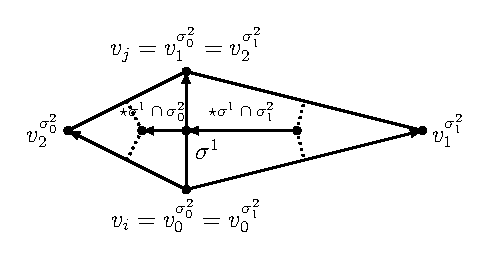
\includegraphics[width=.45\textwidth]{bilder/tikz/elementSummeKante.eps}
          \caption{Two adjacent (triangle) elements share a common edge \( \sigma^{1}=\left[ v_{i}, v_{j} \right] \).
                   The vertices are local indexed on these elements.}
          \label{figLocalIndexing}
        \end{figure}
        Hence we can extract from \eqref{eqLokalLaplace} a local coefficients matrix
        \begin{align}
          A^{\sigma^{2}} 
              &:= {\footnotesize\begin{bmatrix}
                    -\left( C^{\sigma^{2}}_{01} + C^{\sigma^{2}}_{02}\right) & C^{\sigma^{2}}_{01} & C^{\sigma^{2}}_{02} \\
                    C^{\sigma^{2}}_{01} & -\left( C^{\sigma^{2}}_{01} + C^{\sigma^{2}}_{12}\right) & C^{\sigma^{2}}_{12} \\
                    C^{\sigma^{2}}_{02} & C^{\sigma^{2}}_{12} & -\left( C^{\sigma^{2}}_{02} + C^{\sigma^{2}}_{12}\right)
                  \end{bmatrix}} 
        \end{align}
        which holds all computation parts for the local vertices.
        All \( A^{\sigma^{2}} \) can be assembly in a familiar way to get a sparse global matrix 
        \( A\in\R^{N_{\sigma^{0}} \times N_{\sigma^{0}}} \), where \( N_{\sigma^{0}} \) are the number of vertices in \( K \).
        At the end, for \( f_{h}\in\R^{N_{\sigma^{0}}} \), the vector of evaluations for \( f \) 
        (resp. vector of DOFs\footnote{Degree Of Freedom}), 
        \( Af_{h} \) is the result of \eqref{eqVoronoiLaplace} on all global vertices.

        The great advantage of this proceeding is the compatibility to existing Finite Element code 
        like AMDiS\footnote{Adaptive MultiDimensional Simulation toolbox, developed at Institute for Scientific Computing, TU-Dresden}
        \cite{amdis}.
        Only the element operator \( A^{\sigma^{2}} \) must be implemented 
        under use of linear test functions for the interpolation. 
        All other works, like mesh management, problem formulation on the user level, assembling and solving of the linear System, 
        can be done by the FE-toolbox.

    \subsubsection{The discrete gradient}
      The gradient of a scalar valued function \( f \) can be obtained by rising the indices of its exterior derivative, 
      in other words \( \nabla f = \left( \exd f \right)^{\sharp} \).
      Unfortunately, the sharp operator \( \sharp \) depends on the (unknown) metric of the manifold. 
      In \cite{hirani} it is suggested to use the following discrete sharp operator for such a exact \mh{1}{form} \( \exd f \) to get a discrete
      gradient:
      \begin{align}
        \label{eqGradientHeine}
        \left\langle \left( \exd f \right)^{\sharp} , \star\sigma^{2}\right\rangle
          &:= \sum_{\sigma^{0}\prec\sigma^{2}} \left( f(\sigma^{0}) - f(w) \right) \nabla_{\R^{3}}\Phi_{\sigma^{0}}^{\sigma^{2}} \formkomma
      \end{align}
      with a arbitrary vertex \( w\prec\sigma^{2} \),
      \( \Phi_{\sigma^{0}}^{\sigma^{2}} \) is the linear test function (hat function) for the vertex \( \sigma^{0} \) 
      restricted to \( \sigma^{2} \) and \( \nabla_{\R^{3}} \) is the usual \( \R^{3} \) gradient in the ambient space. 
      The formulation for the \( \R^{3} \) vector \( \left( \exd f \right)^{\sharp} \) is to read component wise 
      as a \( \R^{3} \)-vectorized scalar formulation.
      \eqref{eqGradientHeine} gives us a tangential vector of the polytop \( |K| \) on the circumcenter of the triangle \( \sigma^{2} \).
      But in our setting we want to use a gradient on a vertex of the primal mesh, resp. interpreted on the associated Voronoi cell.
      A simple way to get such a discrete gradient, is to average \eqref{eqGradientHeine} over all dual vertices of the Voronoi cell
      related to the primal vertex \( v \):
      \begin{align} \label{eqGradientAverage}
        \left\langle *\overline\nabla f, \star v \right\rangle
            = \sum_{\sigma^{2}\succ v} \left| \star v \cap \sigma^{2} \right|
                 \sum_{\sigma^{0}\prec\sigma^{2}} \left( f(\sigma^{0}) - f(v) \right) \nabla_{\R^{3}}\Phi_{\sigma^{0}}^{\sigma^{2}}
      \end{align}
      The drawback of the discrete average gradient, which we will use in section \ref{secWeingarten}, is that \( |K| \) has no tangential
      space on its vertices, because the polytop is not continuous differentiable in \( v \).
      This makes the situation for a numerical analysis slightly difficult.
      But comparing calculations for several manifolds and functions and 
      the results in section \ref{secResults} indicate the consistence of \eqref{eqGradientAverage} to the smooth
      gradient, 
      if the triangulation is fine enough. 
      
      \paragraph{Note on Implementation}
        Like in section \ref{secDisLaplaceBeltrami}, we can deploy a coefficients matrix for the \mh{q}{th} component of 
        \eqref{eqGradientAverage} for a triangle \( \sigma^{2} \):
        \begin{align}
            \begin{bmatrix}
              -\left( C^{\sigma^{2}}_{01q} + C^{\sigma^{2}}_{02q}\right) & C^{\sigma^{2}}_{01q} & C^{\sigma^{2}}_{02q} \\
              C^{\sigma^{2}}_{10q} & -\left( C^{\sigma^{2}}_{10q} + C^{\sigma^{2}}_{12q}\right) & C^{\sigma^{2}}_{12q} \\
              C^{\sigma^{2}}_{20q} & C^{\sigma^{2}}_{21q} & -\left( C^{\sigma^{2}}_{20q} + C^{\sigma^{2}}_{21q}\right)
            \end{bmatrix}
        \end{align}
        with 
        \begin{align}
          C^{\sigma^{2}}_{klq} &:= \left| \star v_{k}^{\sigma^{2}} \cap \sigma^{2} \right|
                                   \frac{\partial}{\partial x^{q}} \Phi^{\sigma^{2}}_{v_{l}^{\sigma^{2}}} \formkomma
        \end{align}
        for \( k,l,q\in\left\{ 0,1,2 \right\} \) 
        and \( \left( x^{0}, x^{1}, x^{2} \right) \) are the ordinary \( \R^{3} \) coordinates.

        



      
\section{Curvature approximations}
  \subsection{Curvature vector} \label{secCurvatureVector}
    The curvature vector \( \vec{H} \) is given by
    \begin{align}\label{eqMeanCurvCurvVec}
      \vec{H} = 2 H \vec{\nu}
    \end{align}
    for the mean curvature \( H \) and normals \( \vec{\nu} \). 
    In this paper, the mean curvature is set as the arithmetic mean of the two principal curvatures and
    \( H \) should be all over positive for a sphere (i.e. \( H\equiv1 \) on \( \mathds{S}^{2} \)).
    \( H \) and \( \vec{H} \) are extrinsic curvature values.
    This means, that an two dimensional ``inhabitant'' of the surface can't determine this kind of curvature 
    in contrast to the Gaussian curvatures.
    With the inclusion map \( \vec{x}:= \R^{3}\supset M \hookrightarrow \R^{3} \), which is the position vector of \( M \) in \( \R^{3} \),
    the curvature vector can be calculated by (see \cite[Ch. 5]{chen}, \cite[Ch. 4.5]{flanders} or \cite{elliott})
    \begin{align} \label{eqCurvatureVector}
      -\Delta_{B}\vec{x} = \vec{H} \formpunkt
    \end{align}
    (Note that \( \vec{x} \) is an isometric immersion with the common induced metric from \( \R^{3} \).)

    The equation \eqref{eqCurvatureVector} is to read component-wise and can be discretized with 
    the discrete Laplace-Beltrami operator in \eqref{eqDisLaplace}, 
    where \( f \) becomes the \mh{i}{th} coordinate functions \( x^{i} \) for
    \( i=0,1,2 \).
    I.e. we solve for all vertices \( v\in K \) and \( i=0,1,2 \).
    \begin{align} \label{eqDisCurvatureVector}
      \left\langle *\Delta_{B} x^{i}, \star v \right\rangle
        &= \left\langle *H^{i}_{LX}, \star v \right\rangle \formpunkt
    \end{align}
    \( H^{i}_{LX}\in \R \) are the components of the approximated curvature vector.
    The right-hand side (RHS) of \eqref{eqDisCurvatureVector} can be locally represented by the decomposed Voronoi area 
    \begin{align}
      C^{\sigma^{2}}_{i} = \left| \star v \cap \sigma^{2}  \right|
    \end{align}
    around \( v\prec\sigma^{2} \).
    Hence, the local coefficients matrix of the RHS of \eqref{eqDisCurvatureVector}
    (and generally for all Zero-Order-Terms of scalar valued functions) becomes
    \begin{align}
      \begin{bmatrix}
        C^{\sigma^{2}}_{0} & 0 & 0 \\
        0 & C^{\sigma^{2}}_{1} & 0 \\
        0 & 0 & C^{\sigma^{2}}_{2}
      \end{bmatrix}
    \end{align}
    and can be assembly in a common way.

    The mean curvature \( H \) is determined with \eqref{eqMeanCurvCurvVec} by taking the euclidean \mh{\R^{3}}{norm}
    \begin{align}
      H_{LX} = \frac{s}{2}\left\| \vec{H}_{LX} \right\|_{\R^{3}}
    \end{align}
    on every vertex with respect to the sign \( s:K^{(0)}\rightarrow\left\{ +1,-1 \right\} \),
    which depends on the direction of \(  \vec{H}_{LX} \).
    If the approximated curvature vector point outward the polytop \( K \), then is \( s=+1 \) and vice versa. 

    
    


  \subsection{Weingarten map} \label{secWeingarten}
    The Weingarten map (shape operator) \( S \)
    can be obtained by rising on time the indices of the second fundamental form \( \II \)
    (see \cite{FirstCourse}),
    i.e. \( S = (g)^{-1}\II \) with a metric tensor \( g \),
    or by the exterior derivatives of the normal components:
    \begin{align}
    \begin{aligned}\label{eqDefWeingarten}
      S: T_{\vec{x}}M &\rightarrow T_{\vec{x}}M \\
                    \vec{w} &\mapsto \exd\vec{\nu} \left( \vec{w} \right) \formpunkt
    \end{aligned}
    \end{align}
    In particularly, \( \exd\nu^{i} \left( \vec{w} \right) \) is the directional derivative of the \mh{i}{th} normal component \( \nu^{i} \) 
    along \( \vec{w} \).
    The eigenvalues of \( S \) are the principal curvatures \( \kappa_{1} \) and \( \kappa_{2} \).
    Note that the linear operator \( S \) by \eqref{eqDefWeingarten} as matrix have a column space in local coordinates 
    and depends on the choice of the parametrisation as a consequence.
    A more manageable formulation is the extended Weingarten map
    \begin{align}\label{eqDefExWeingarten}
      \bar{S}:= \nabla\vec{\nu} \formkomma
    \end{align}
    which can be defined on the entire tangential space of the \( \R^{3} \) (if the normal vectors of \( M \) are smoothly extended to them).
    The point is, that \( \bar{S} \), restricted to \( T_{\vec{x}}M \), is the Weingarten map \( S \) (see \cite[Pt. 2, Ch. 2]{kimura}),
    with the additive eigenvalue 0,
    and \eqref{eqDefExWeingarten} can be approximated by our discrete average gradient \eqref{eqGradientAverage},
    i.e. we calculate the \mh{i}{th} row \( \bar{s}_{i}\in\R^{3} \) of the discrete extended Weingarten map \( \bar{S}_{W}\in\R^{3\times 3} \) by
    \begin{align} \label{eqDisWeingarten}
      \left\langle *\overline{\nabla}\nu^{i} , \star v \right\rangle 
        &= \left\langle *\bar{s}_{i} , \star v \right\rangle
    \end{align}
    on all vertices \( v\in K \).
    For numerical reason we symmetrize \( \bar{S}_{W} \) by
    \begin{align}
      \bar{S}_{W}^{Sym} &:= \frac{1}{2}\left( \bar{S}_{W} + \bar{S}_{W}^{T} \right)
    \end{align}
    to get the same property like the smooth extended Weingarten map.
    To obtain the eigenvalues we use the QR-algorithm of the MTL4\footnote{Matrix Template Library 4}.
    The lowest eigenvalue regarding to the absolute value is omitted.
    So w.l.o.g.
    \begin{align}
      \left\{\kappa_{1},\kappa_{2}\right\} &\approx \left\{ \kappa_{W,1}, \kappa_{W,2} \right\} \\ 
                    &:= \left\{ \lambda\in\text{Eig}(\bar{S}_{W}^{Sym}) \middle|\ \exists\lambda_{0}\in\text{Eig}(\bar{S}_{W}^{Sym}): \left| \lambda \right| > \lambda_{0} \right\} 
    \end{align}
    Hence, the approximated Gauss and mean curvatures are
    \begin{align}
      K_{W} &:= \kappa_{W,1} \cdot \kappa_{W,2} \\
      H_{W} &:= \frac{1}{2}\left( \kappa_{W,1} + \kappa_{W,2} \right) \formpunkt
    \end{align}

    The equations \eqref{eqDisWeingarten} can be applied, only if we know the exact normals of the manifolds on the vertices, 
    e.g. if the surface \( M \) is described by the 0-level-set of a signed distance function \( \varphi:\R^{3}\rightarrow\R \),
    then is
    \begin{align}
      \vec{\nu} &= \frac{\nabla_{\R^{3}}\varphi}{\left\| \nabla_{\R^{3}}\varphi \right\|} \formpunkt
    \end{align}
    For arbitrary surface triangulations, where the smooth manifold is unknown, like in figure \ref{figBunnyHorseCurvature},
    we must approximate the normals on the vertices before.
    A simple way to do that, is to average the element normals \( \vec{\nu}^{\sigma^{2}} \) of a triangle \( \sigma^{2}\in K \)
    over the Voronoi area:
    \begin{align}
      \left\langle *\vec{\nu}_{\avn} , \star v \right\rangle
        &:= \sum_{\sigma^{2}\succ v} \left| \star v \cap \sigma^{2} \right| \vec{\nu}^{\sigma^{2}} \formpunkt
    \end{align}
    With the same procedure above, we get the approximated curvatures \( K_{W,\avn} \) and \( H_{W,\avn} \).




\section{Results} \label{secResults}
  
  \begin{align}
    \label{eqSphere}
    \varphi\left( x,y,z \right) &:= x^{2} + y^{2} + z^{2} - 1 \\
    \label{eqEllipsoid}
    \varphi\left( x,y,z \right) &:= \left( 3x \right)^{2} + \left( 6y \right)^{2} + \left( 2z \right)^{2} - 9\\
    \label{eqQuartic}
    \varphi\left( x,y,z \right) &:= \left( x - z^{2} \right)^{2} + \left( y - z^{2} \right)^{2} + z^{2} - 1
  \end{align}


  \begin{figure}
    \centering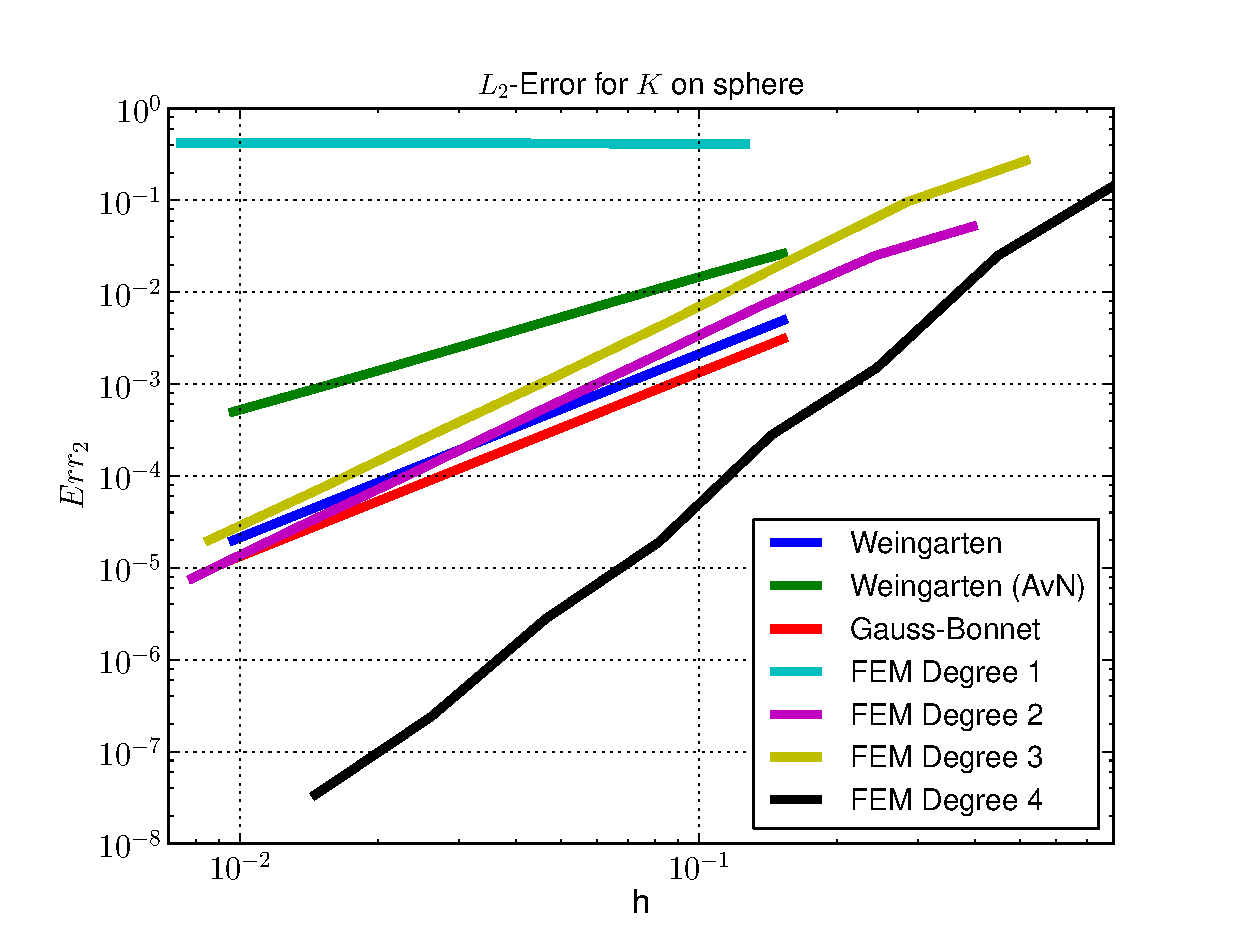
\includegraphics[width=.49\textwidth]{bilder/sphere/L2K.eps}
    \centering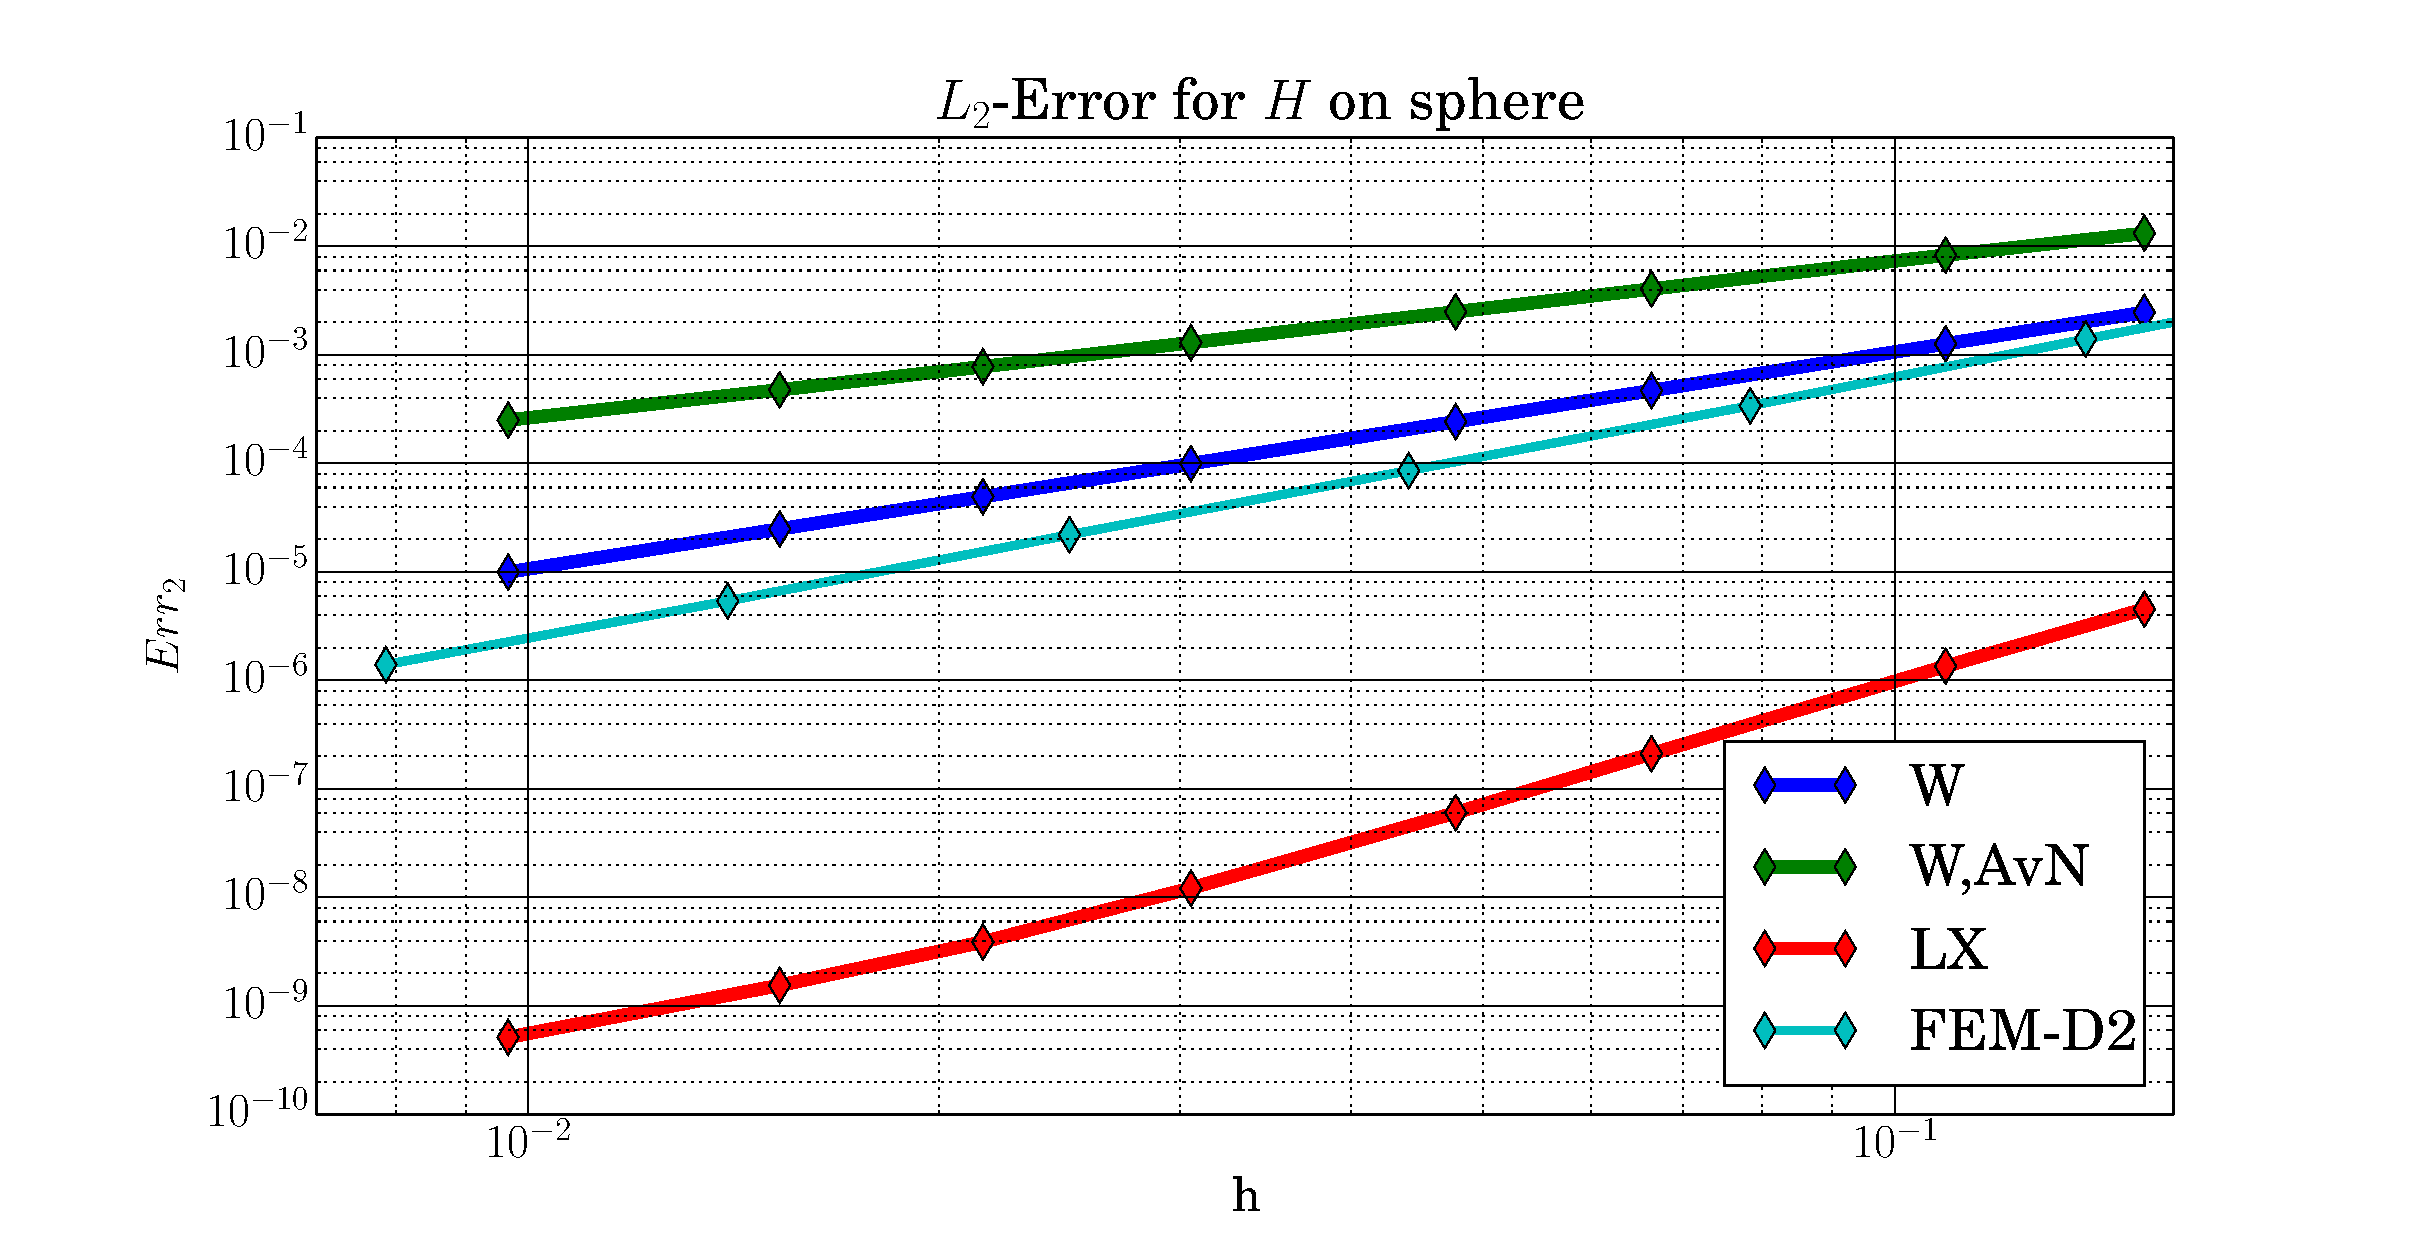
\includegraphics[width=.49\textwidth]{bilder/sphere/L2H.eps}
    \caption{Sphere \eqref{eqSphere}: Relative \( L_{2} \) (top) resp. \( L_{\infty} \) (bottom) error for \( K \) (left) and
                                                     \( H \) (right) for different \( h \) in a log-log-plot.}
    \label{figSphere}
  \end{figure}

  \begin{figure}
    \begin{minipage}[htp]{.23\textwidth}
      \centering
      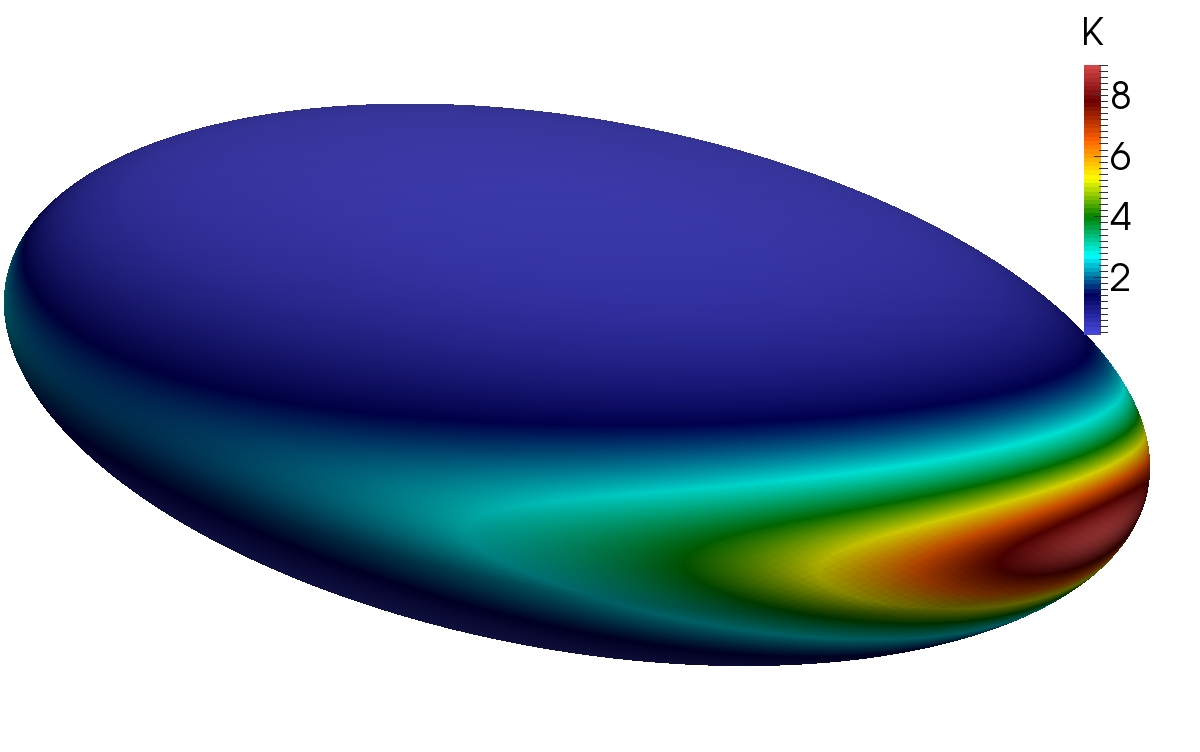
\includegraphics[width=0.99\textwidth]{bilder/ellipsoid/K.jpg}
    \end{minipage}\hfill
    \begin{minipage}[htp]{.23\textwidth}
      \centering
      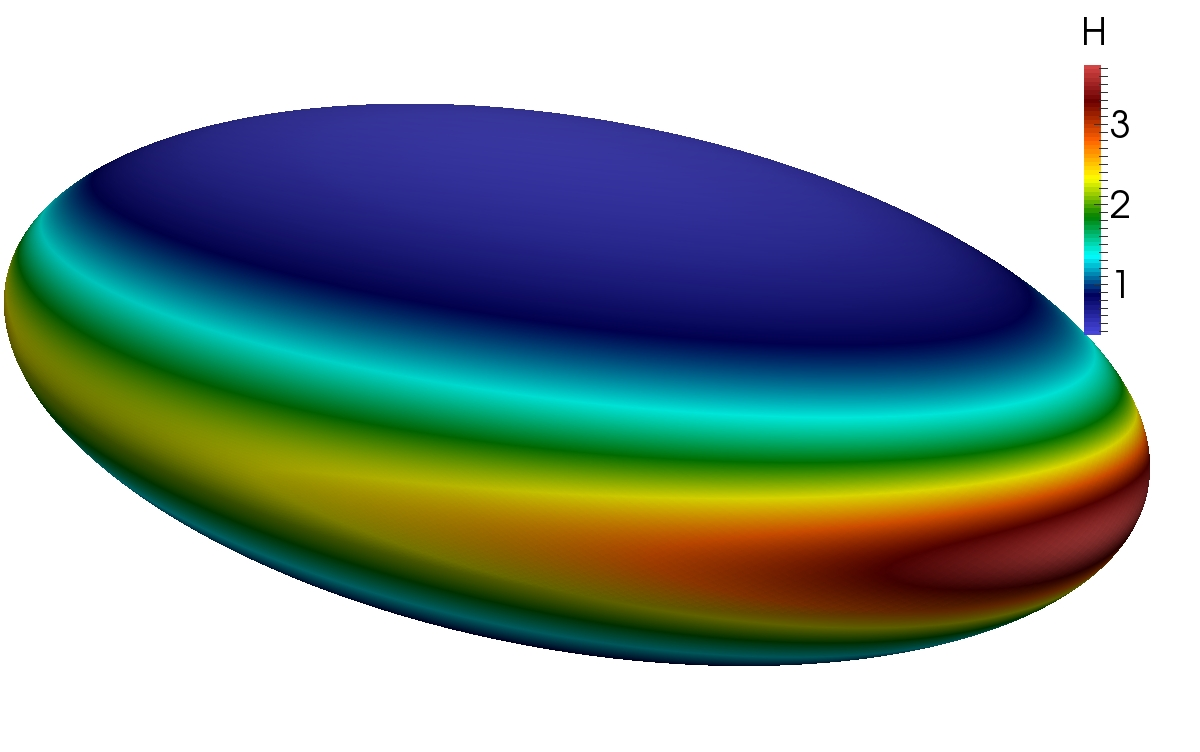
\includegraphics[width=0.99\textwidth]{bilder/ellipsoid/H.jpg}
    \end{minipage}\\
    \begin{minipage}[htp]{.23\textwidth}
      \centering
      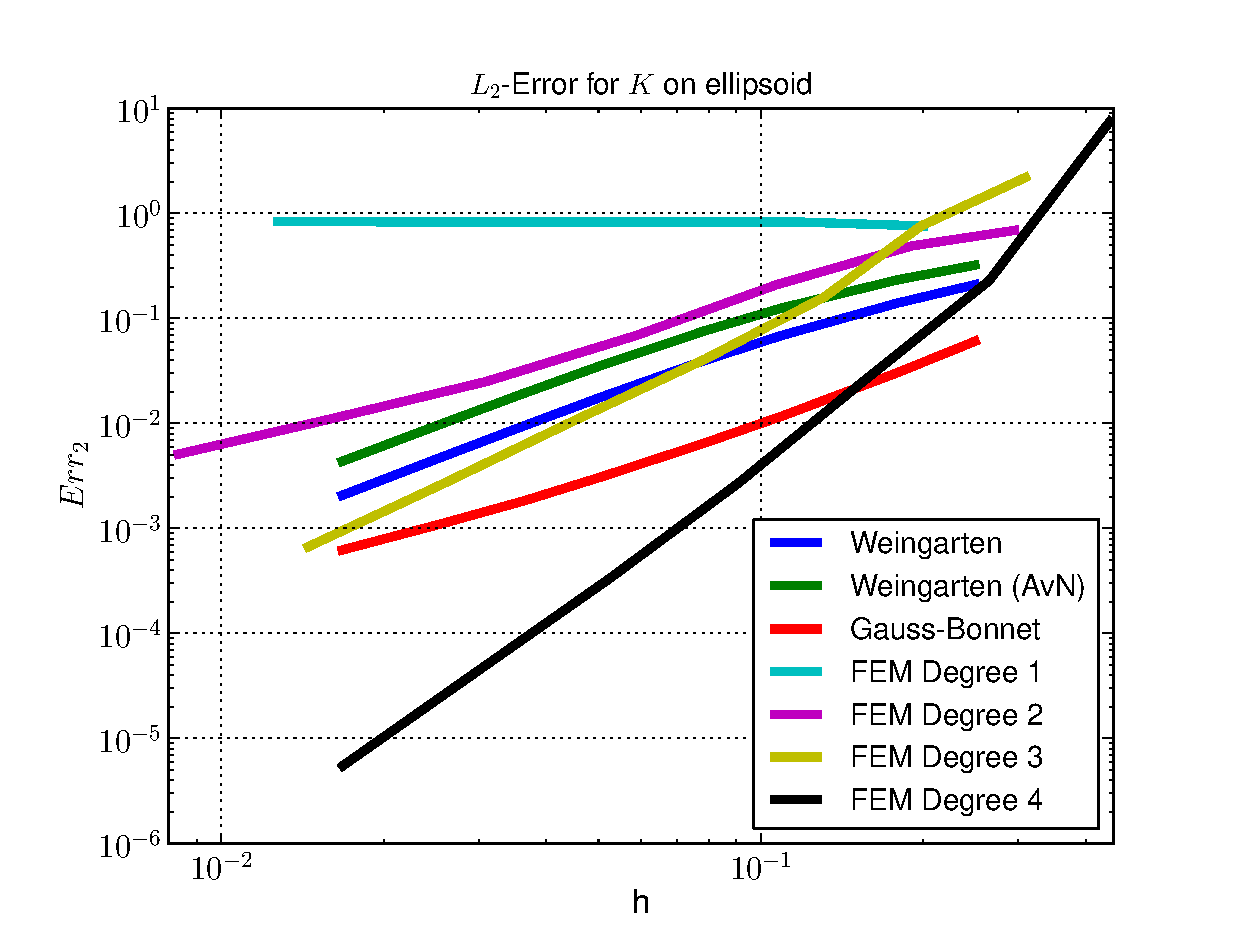
\includegraphics[width=0.99\textwidth]{bilder/ellipsoid/L2K.eps}
    \end{minipage}\hfill
    \begin{minipage}[htp]{.23\textwidth}
      \centering
      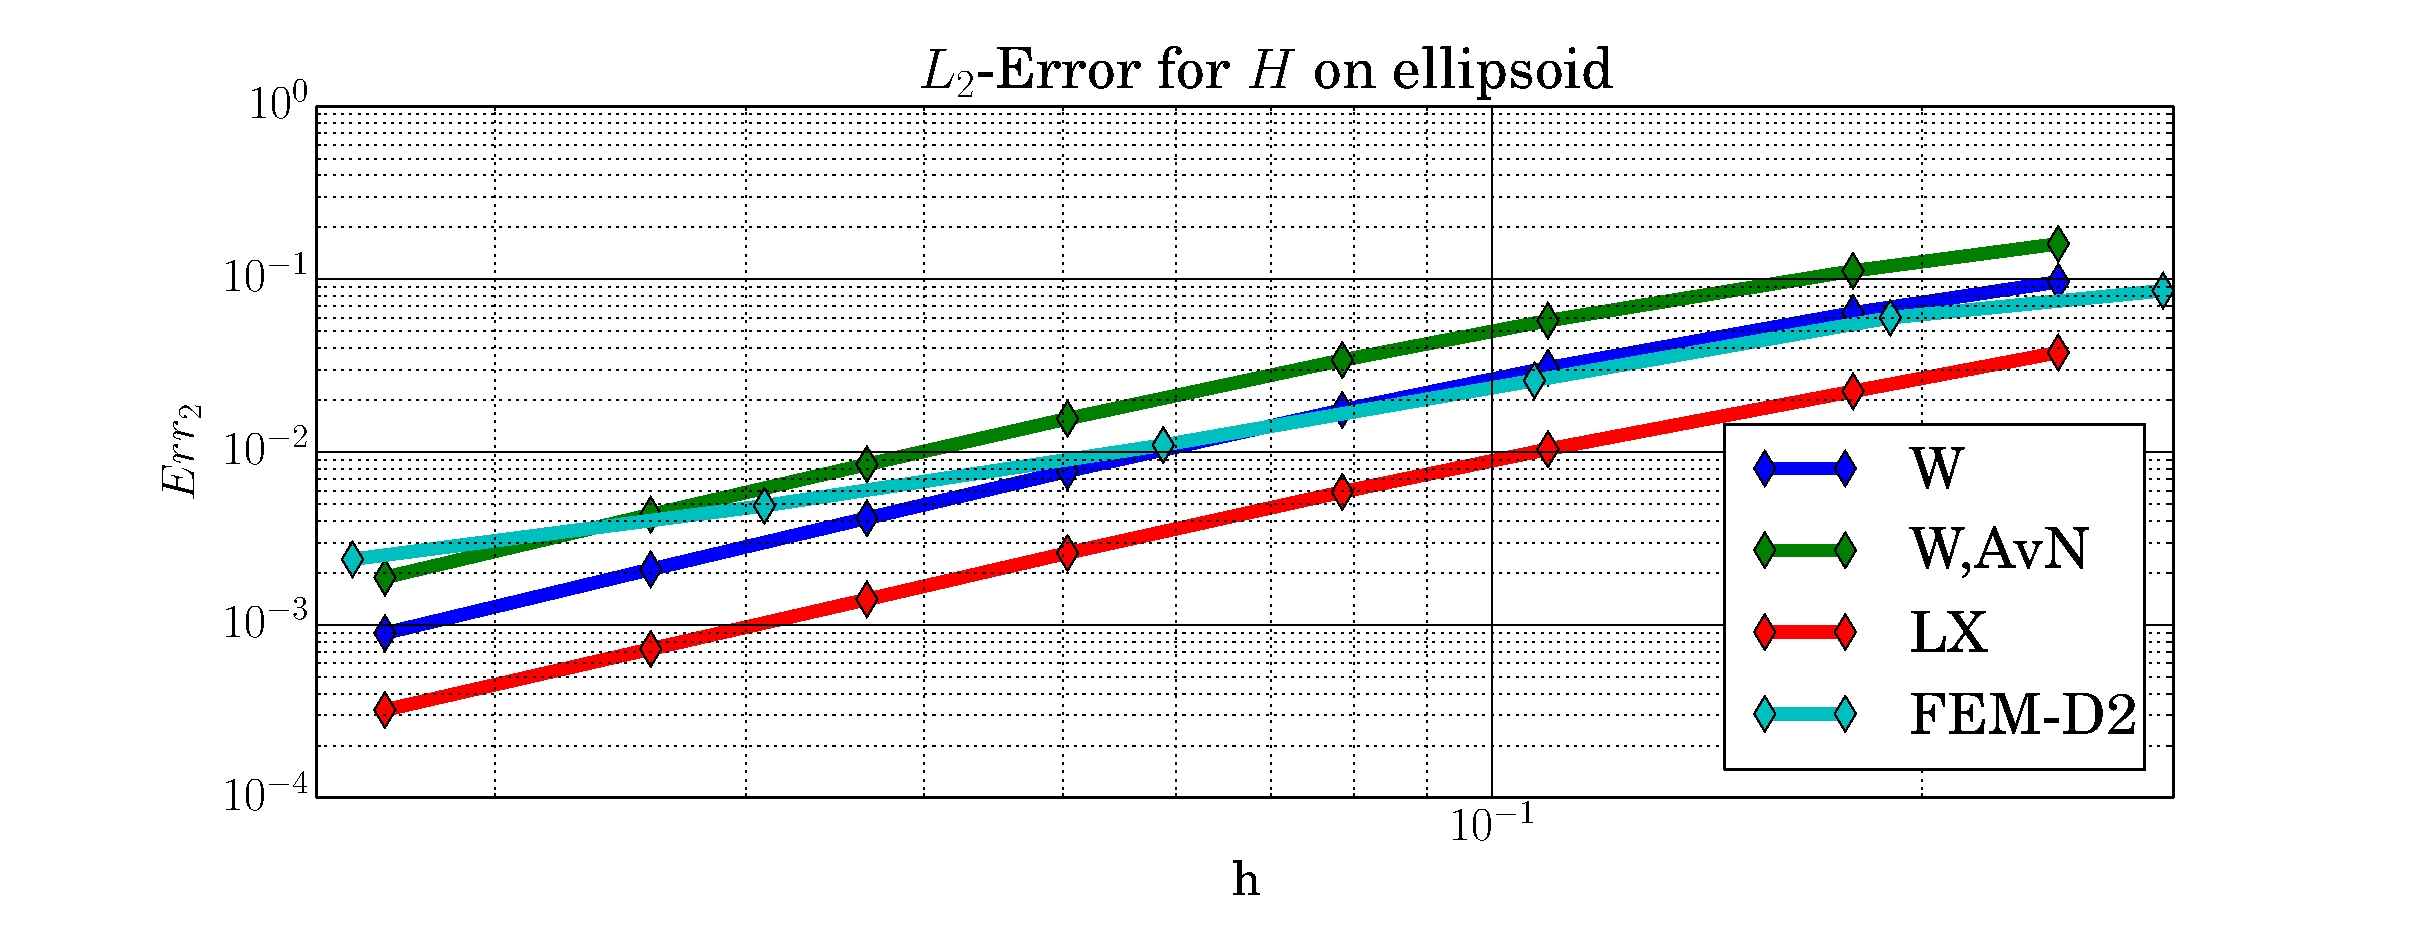
\includegraphics[width=0.99\textwidth]{bilder/ellipsoid/L2H.eps}
    \end{minipage}\\
    \begin{minipage}[htp]{.23\textwidth}
      \centering
      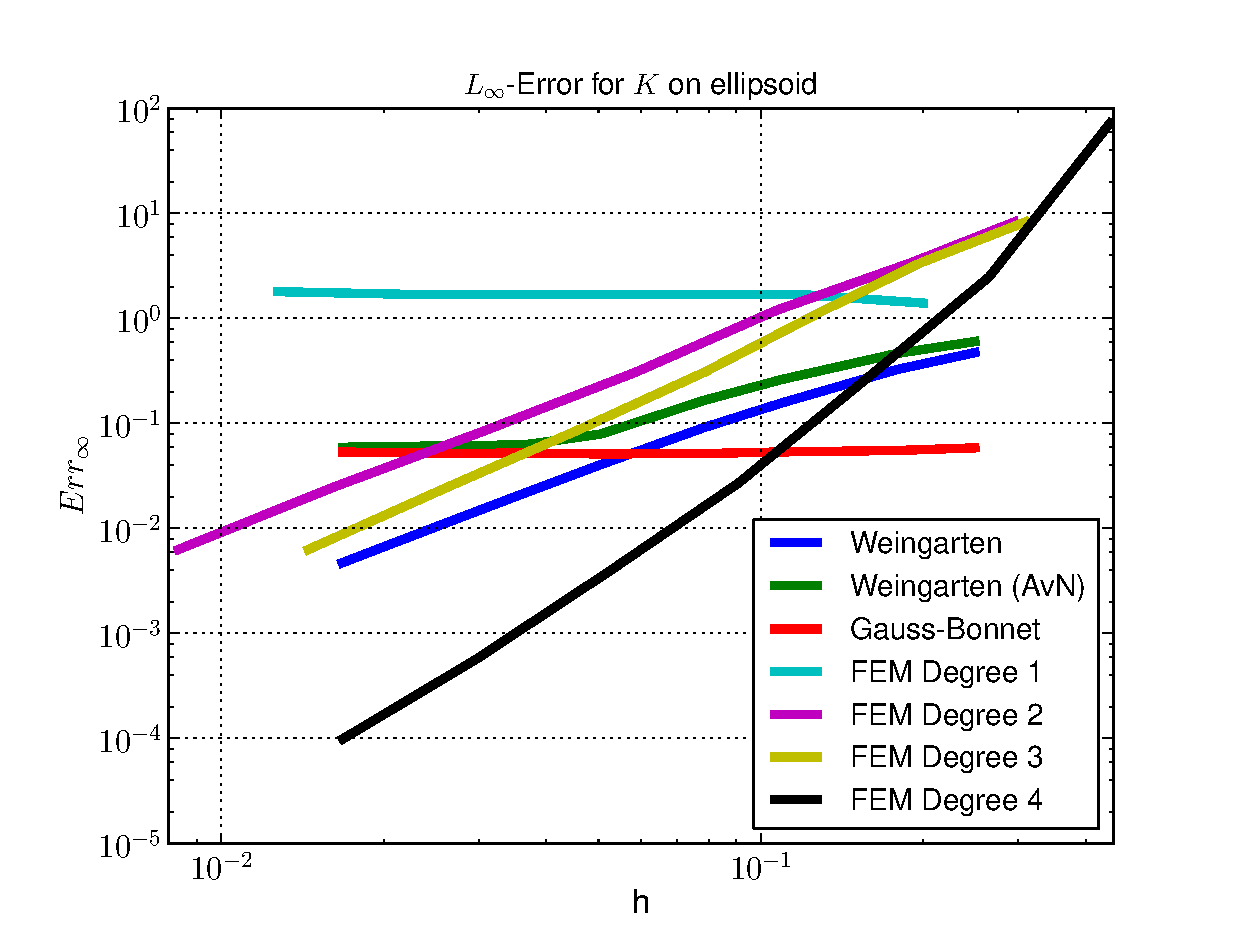
\includegraphics[width=0.99\textwidth]{bilder/ellipsoid/LMaxK.eps}
    \end{minipage}\hfill
    \begin{minipage}[htp]{.23\textwidth}
      \centering
      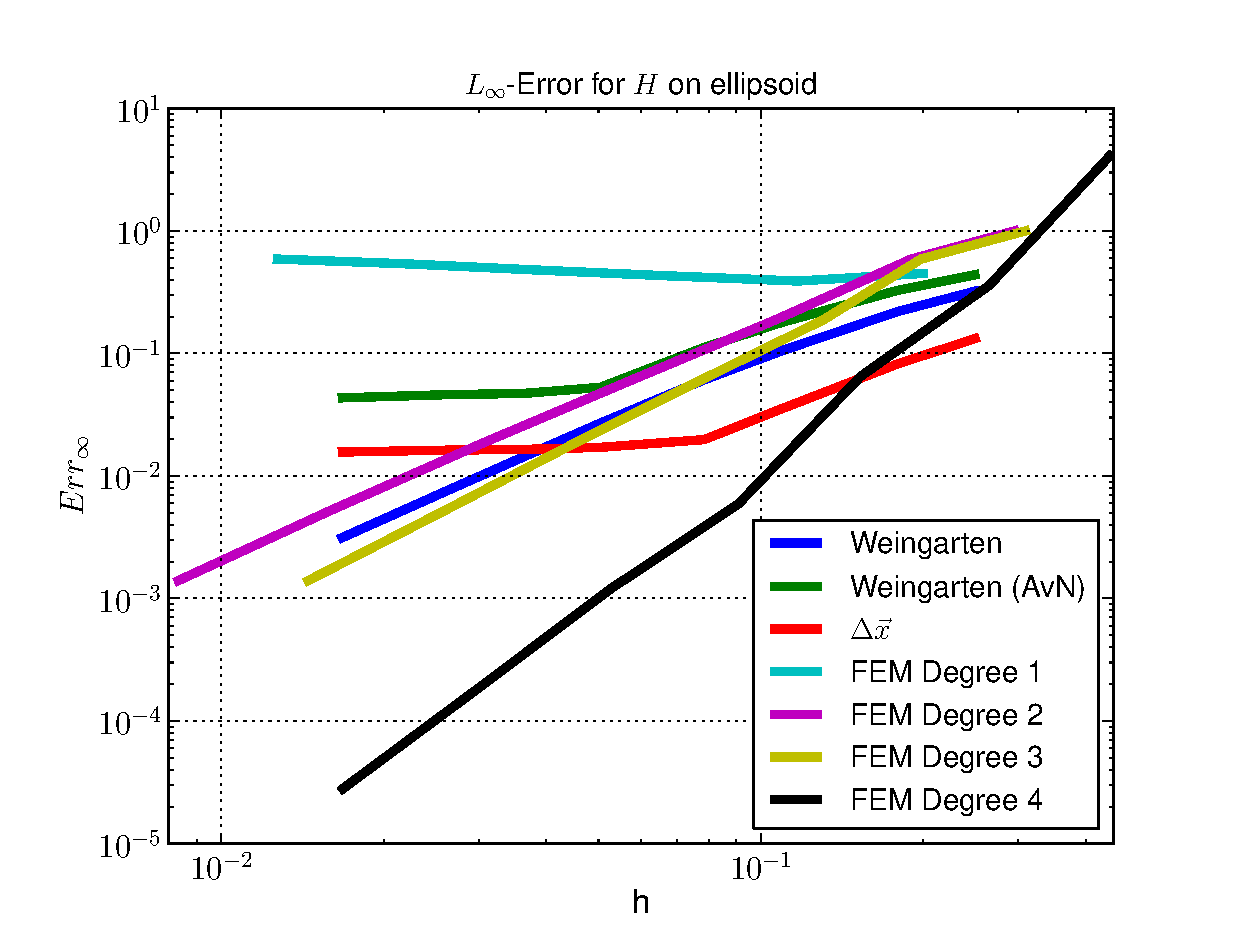
\includegraphics[width=0.99\textwidth]{bilder/ellipsoid/LMaxH.eps}
    \end{minipage}
    \caption{Ellipsoid \eqref{eqEllipsoid}: Top row: Gaussian curvature \( K \) (left) and mean curvature \( H \) (right).
                              Middle and bottom row: Relative \( L_{2} \) resp. \( L_{\infty} \) error for \( K \) (left) and
                                                     \( H \) (right) for different \( h \) in a log-log-plot.}
    \label{figEllipsoid}
  \end{figure}

  \begin{figure}
    \begin{minipage}[htp]{.23\textwidth}
      \centering
      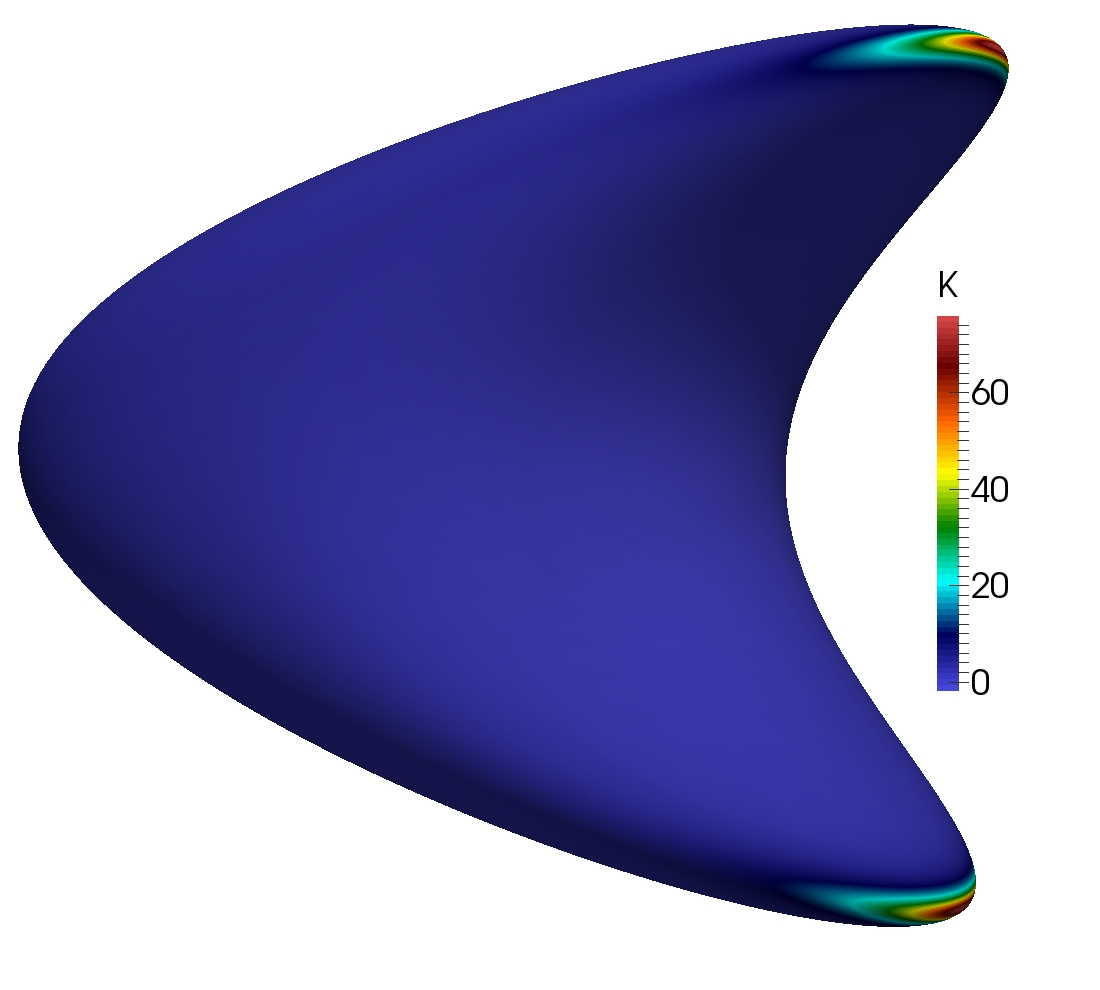
\includegraphics[width=0.99\textwidth]{bilder/quartic/K.jpg}
    \end{minipage}\hfill
    \begin{minipage}[htp]{.23\textwidth}
      \centering
      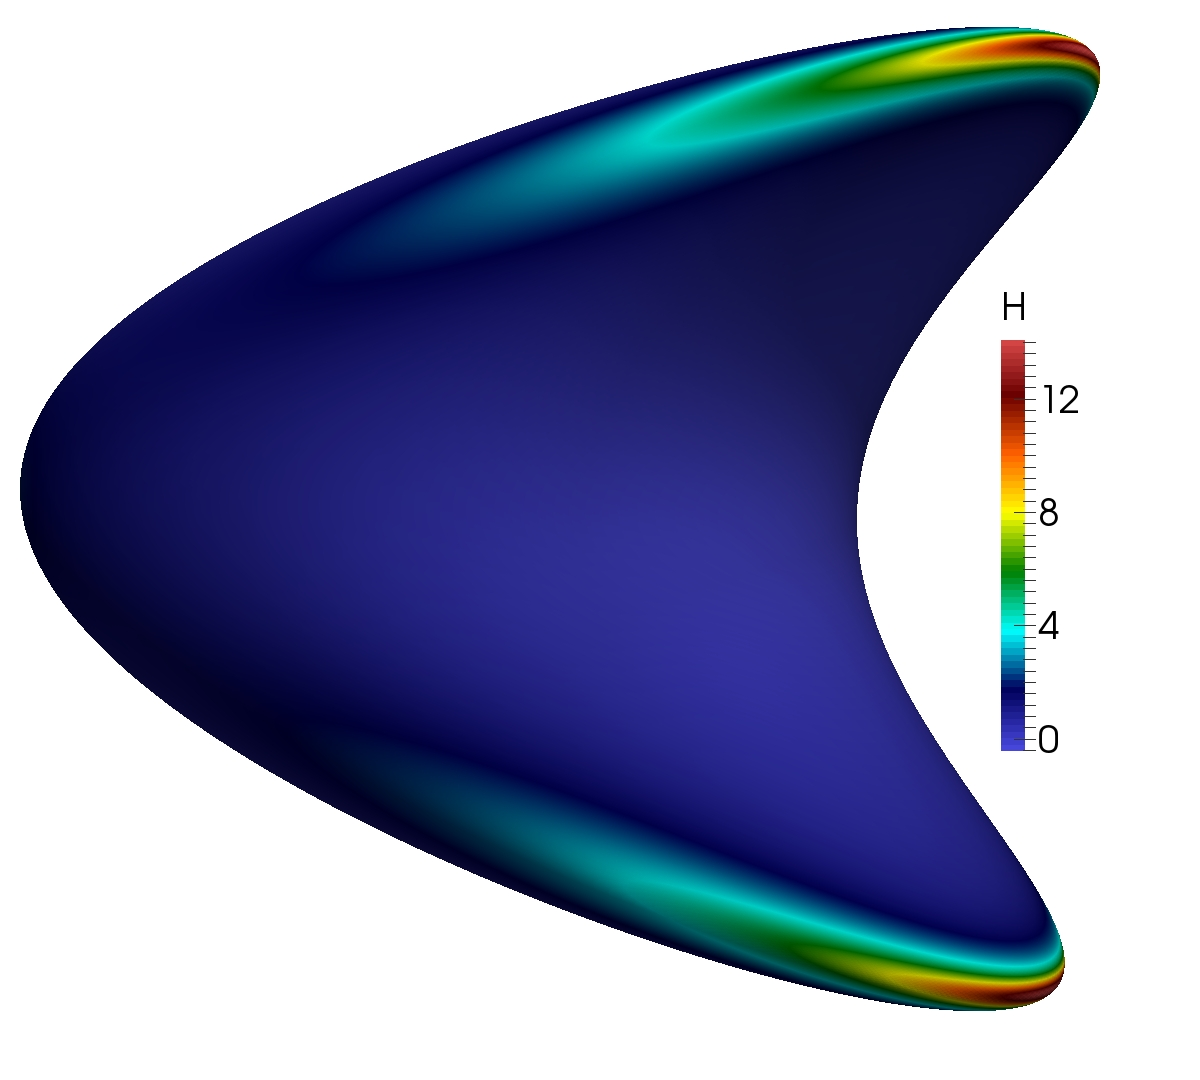
\includegraphics[width=0.99\textwidth]{bilder/quartic/H.jpg}
    \end{minipage}\\
    \begin{minipage}[htp]{.23\textwidth}
      \centering
      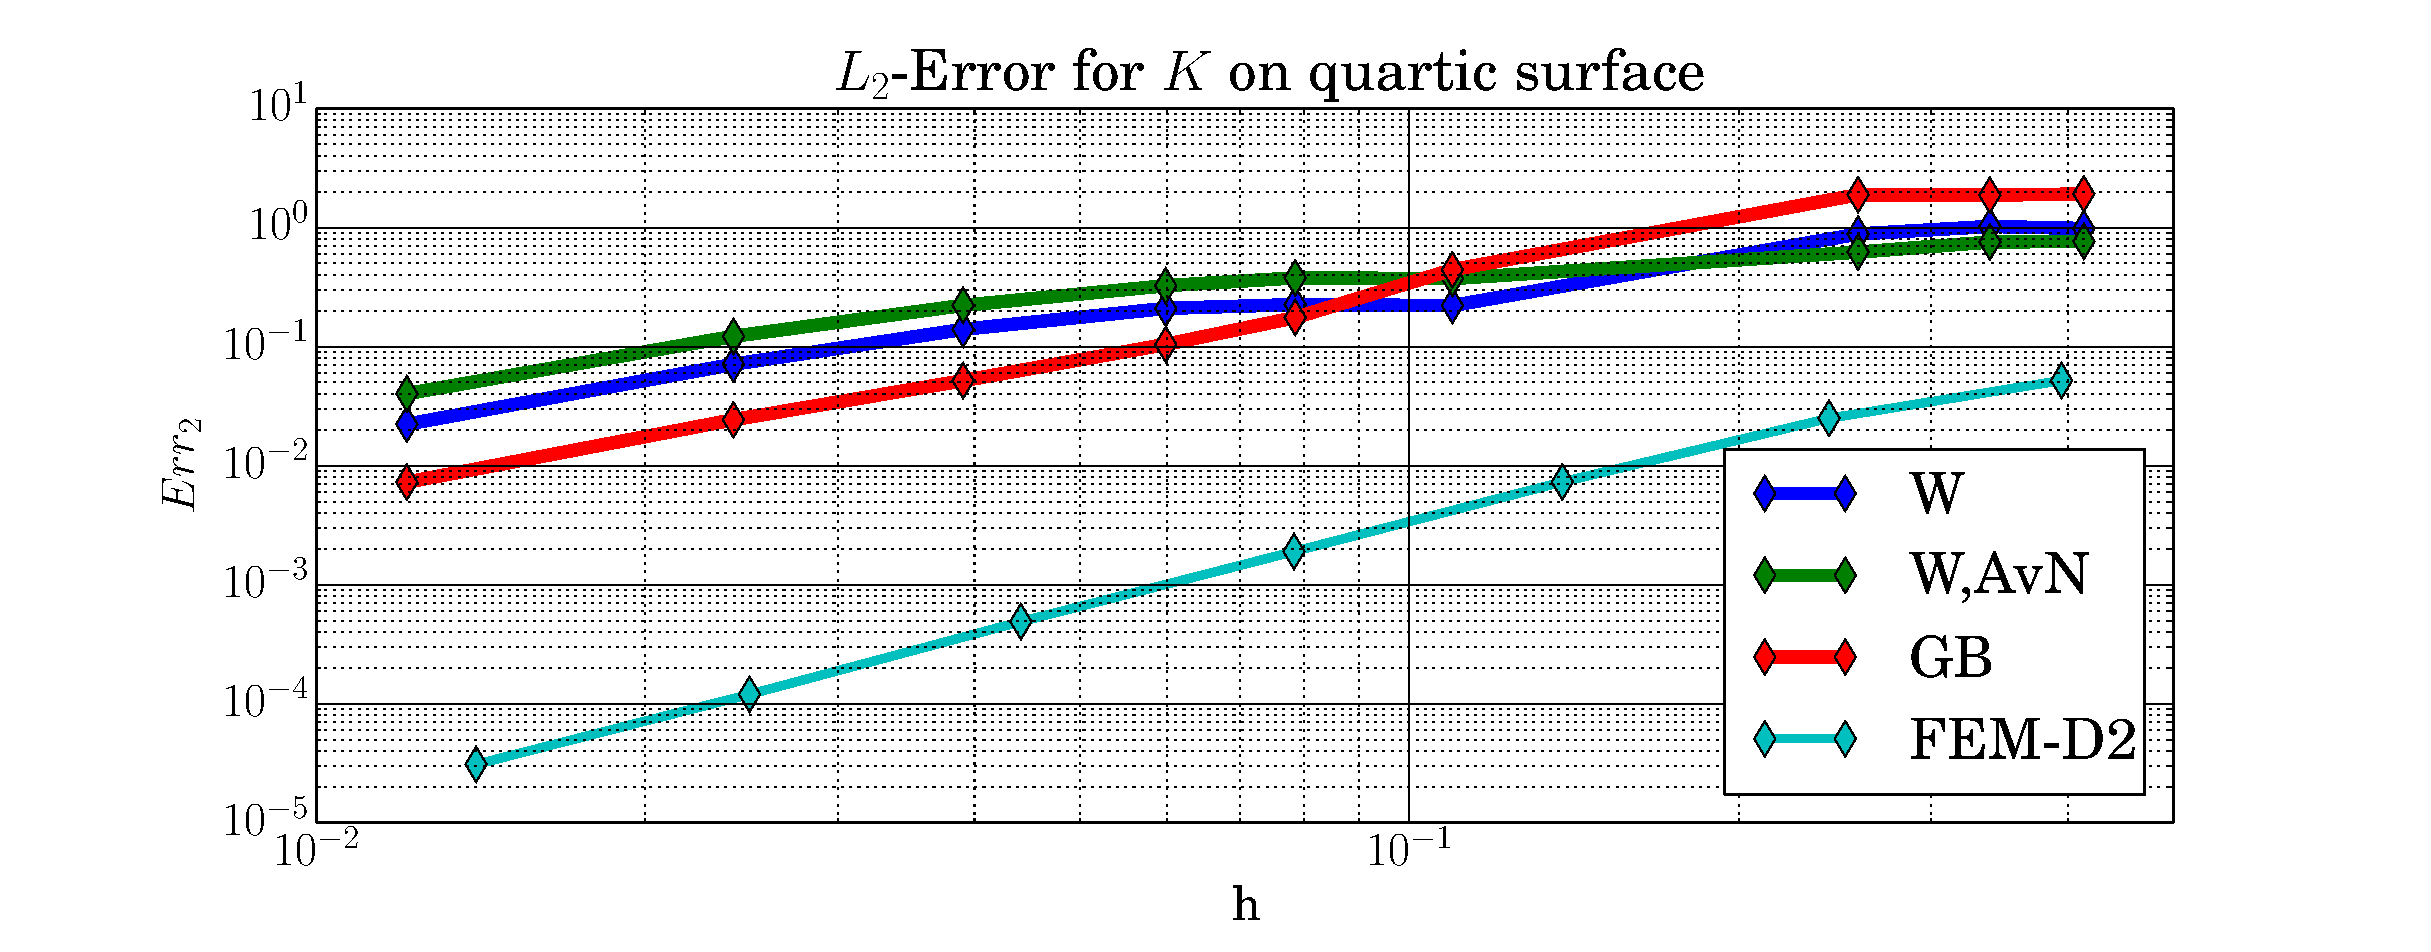
\includegraphics[width=0.99\textwidth]{bilder/quartic/L2K.eps}
    \end{minipage}\hfill
    \begin{minipage}[htp]{.23\textwidth}
      \centering
      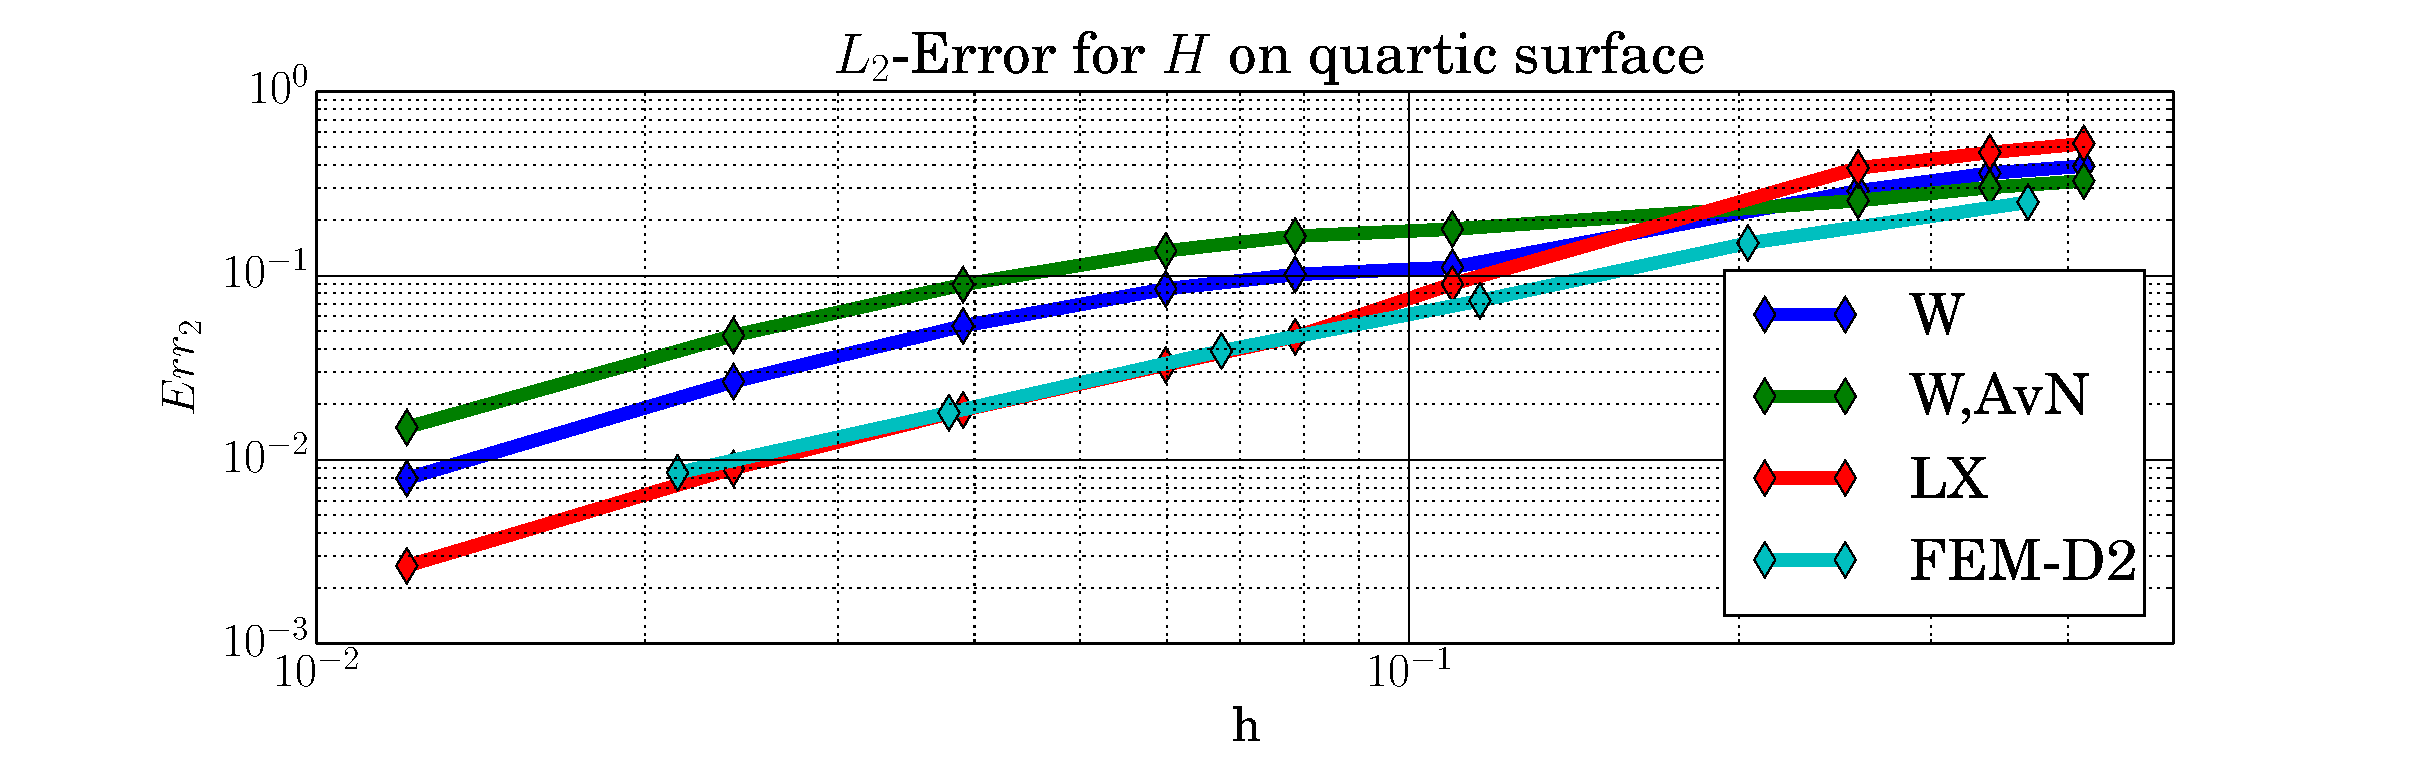
\includegraphics[width=0.99\textwidth]{bilder/quartic/L2H.eps}
    \end{minipage}\\
    \begin{minipage}[htp]{.23\textwidth}
      \centering
      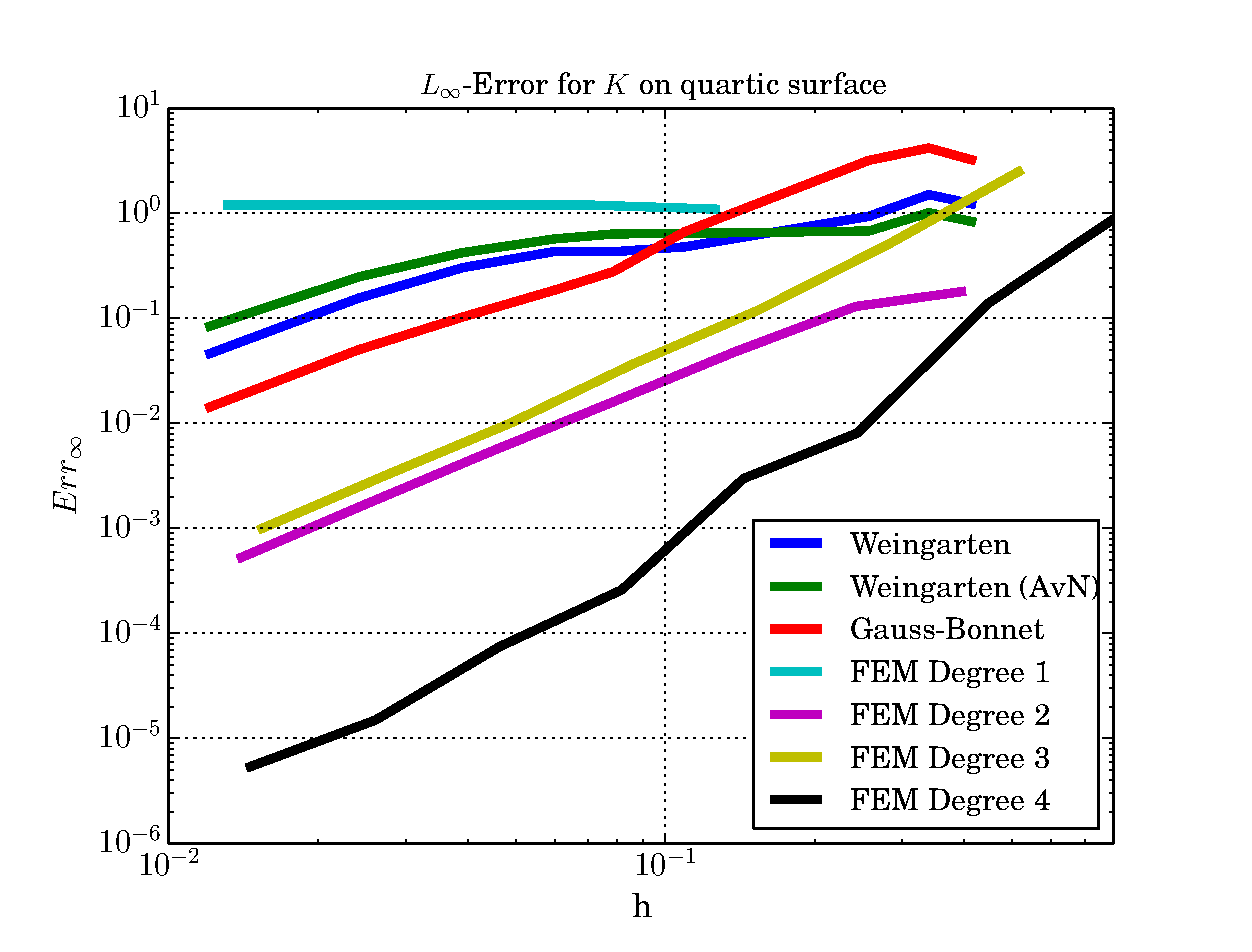
\includegraphics[width=0.99\textwidth]{bilder/quartic/LMaxK.eps}
    \end{minipage}\hfill
    \begin{minipage}[htp]{.23\textwidth}
      \centering
      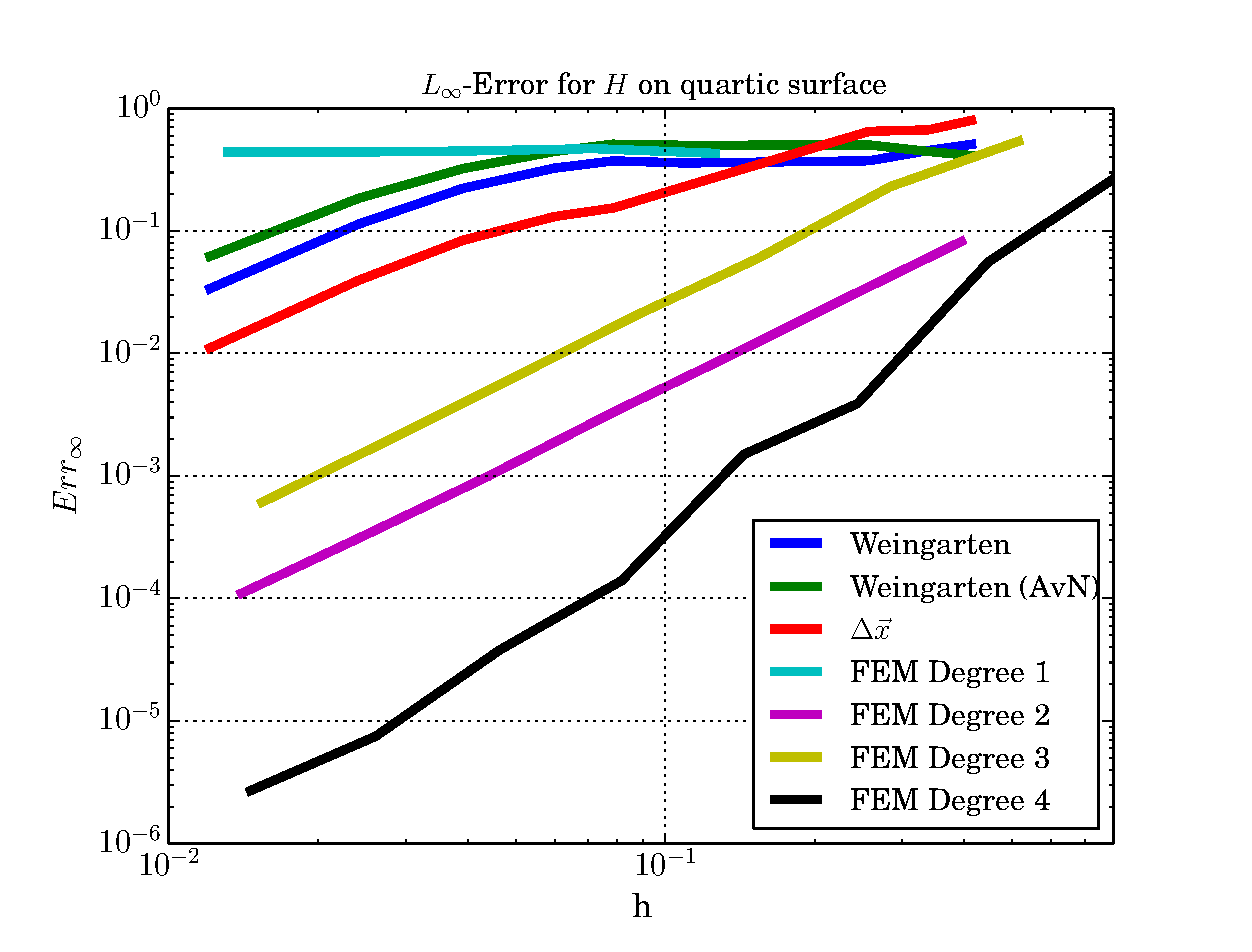
\includegraphics[width=0.99\textwidth]{bilder/quartic/LMaxH.eps}
    \end{minipage}
    \caption{Quartic Surface \eqref{eqQuartic}: Top row: Gaussian curvature \( K \) (left) and mean curvature \( H \) (right).
                              Middle and bottom row: Relative \( L_{2} \) resp. \( L_{\infty} \) error for \( K \) (left) and
                                                     \( H \) (right) for different \( h \) in a log-log-plot.}
    \label{figQuartic}
  \end{figure}

  \begin{figure}
    \begin{minipage}[htp]{.23\textwidth}
      \centering
      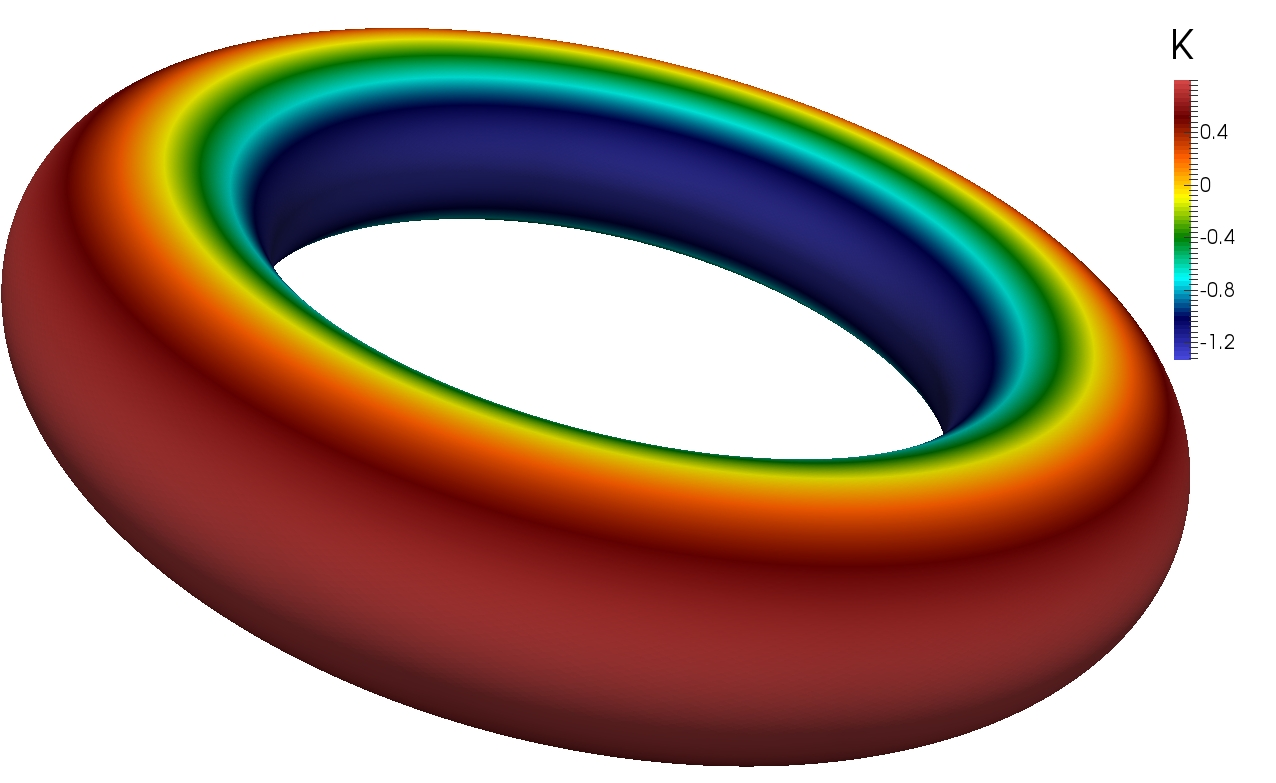
\includegraphics[width=0.99\textwidth]{bilder/torus/K.jpg}
    \end{minipage}\hfill
    \begin{minipage}[htp]{.23\textwidth}
      \centering
      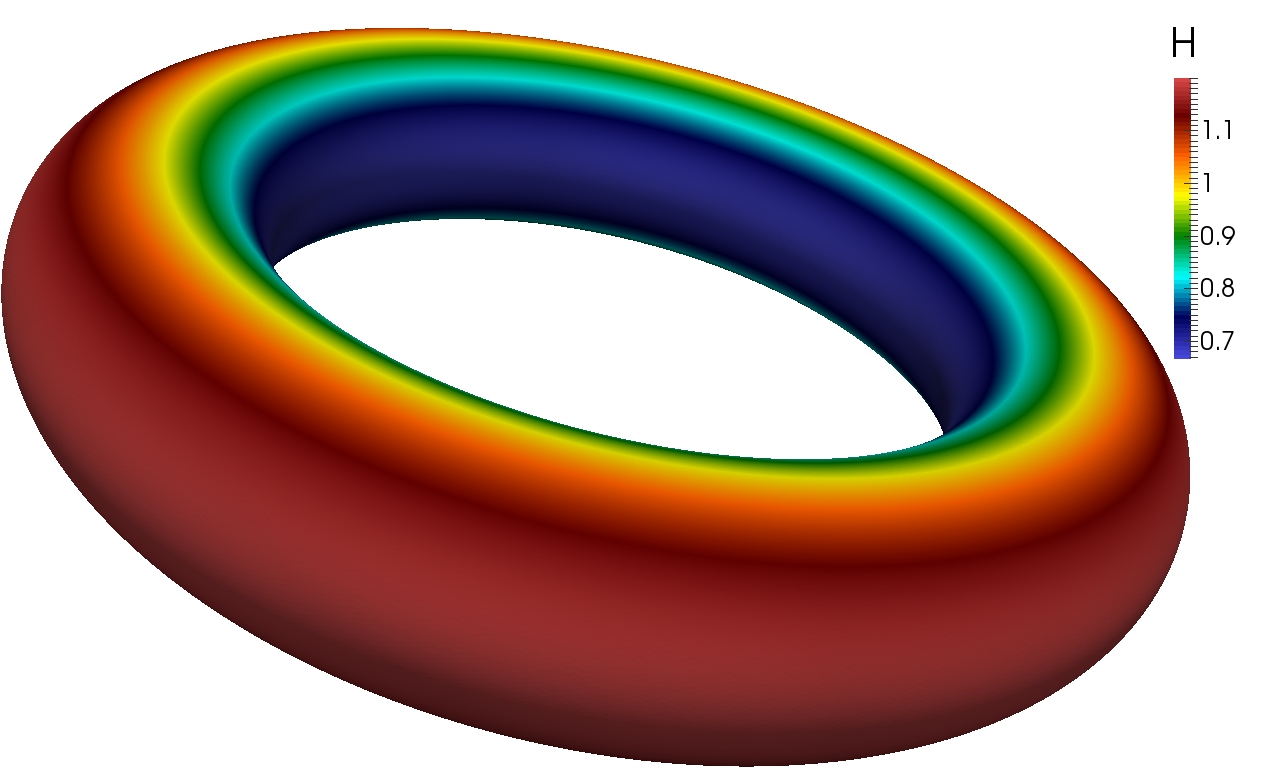
\includegraphics[width=0.99\textwidth]{bilder/torus/H.jpg}
    \end{minipage}\\
    \begin{minipage}[htp]{.23\textwidth}
      \centering
      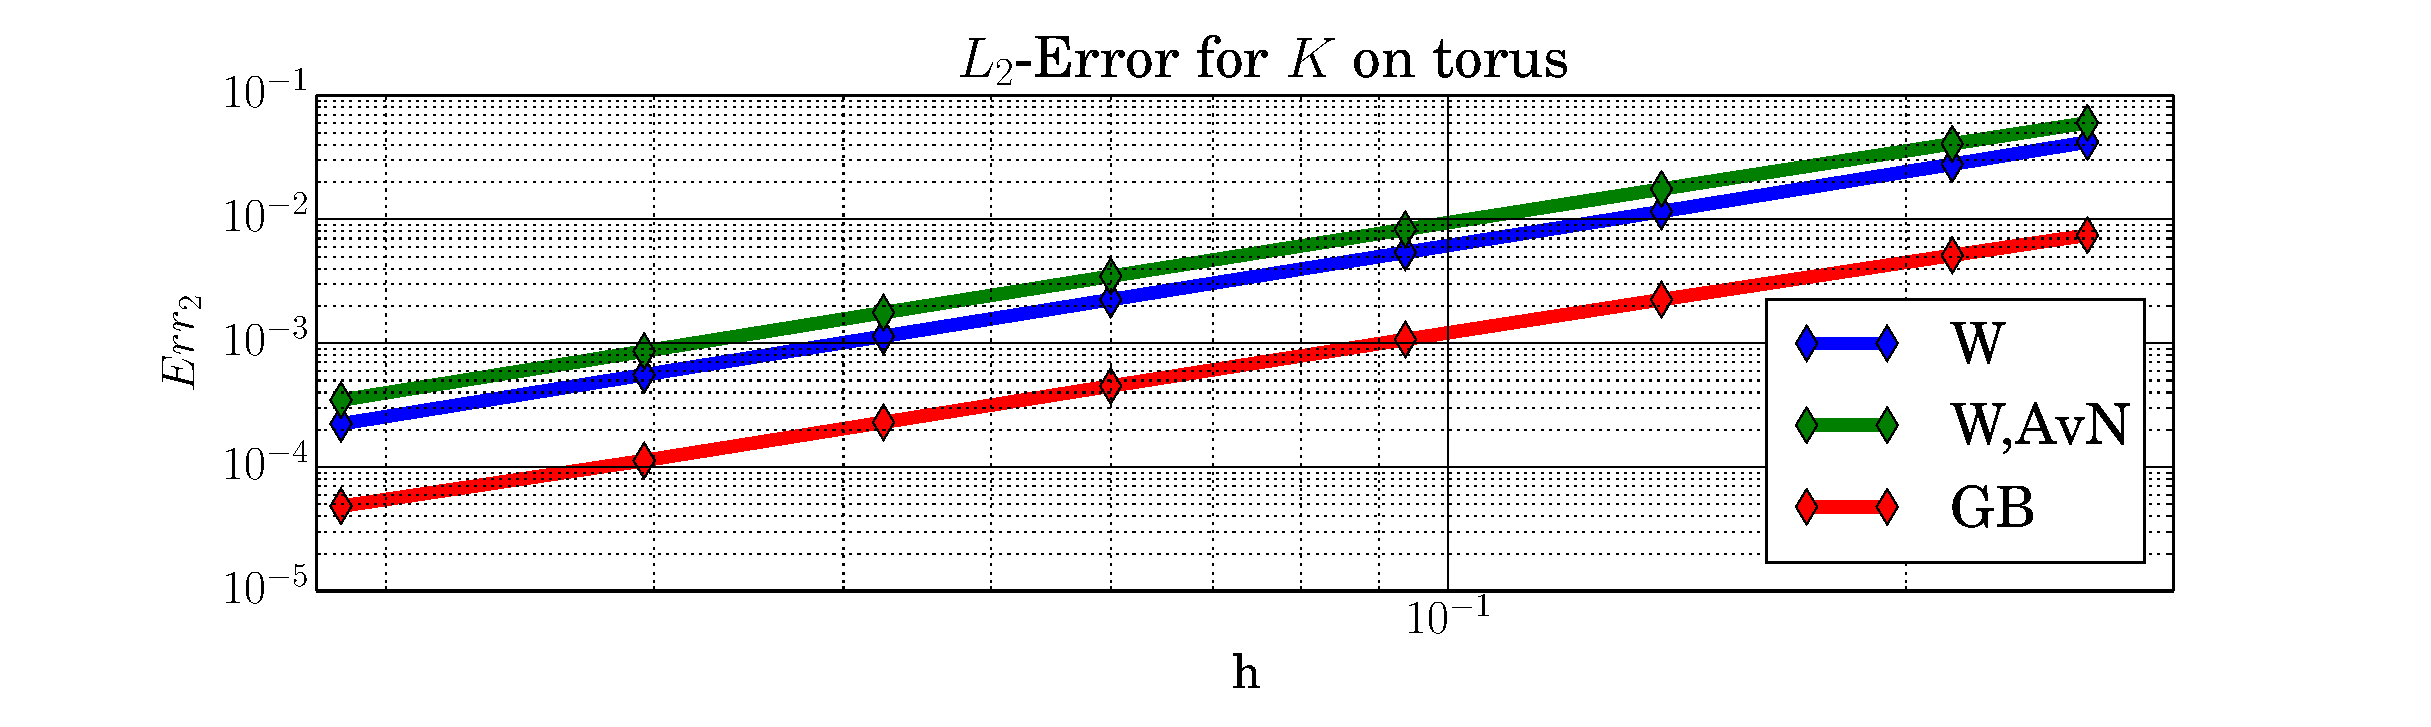
\includegraphics[width=0.99\textwidth]{bilder/torus/L2K.eps}
    \end{minipage}\hfill
    \begin{minipage}[htp]{.23\textwidth}
      \centering
      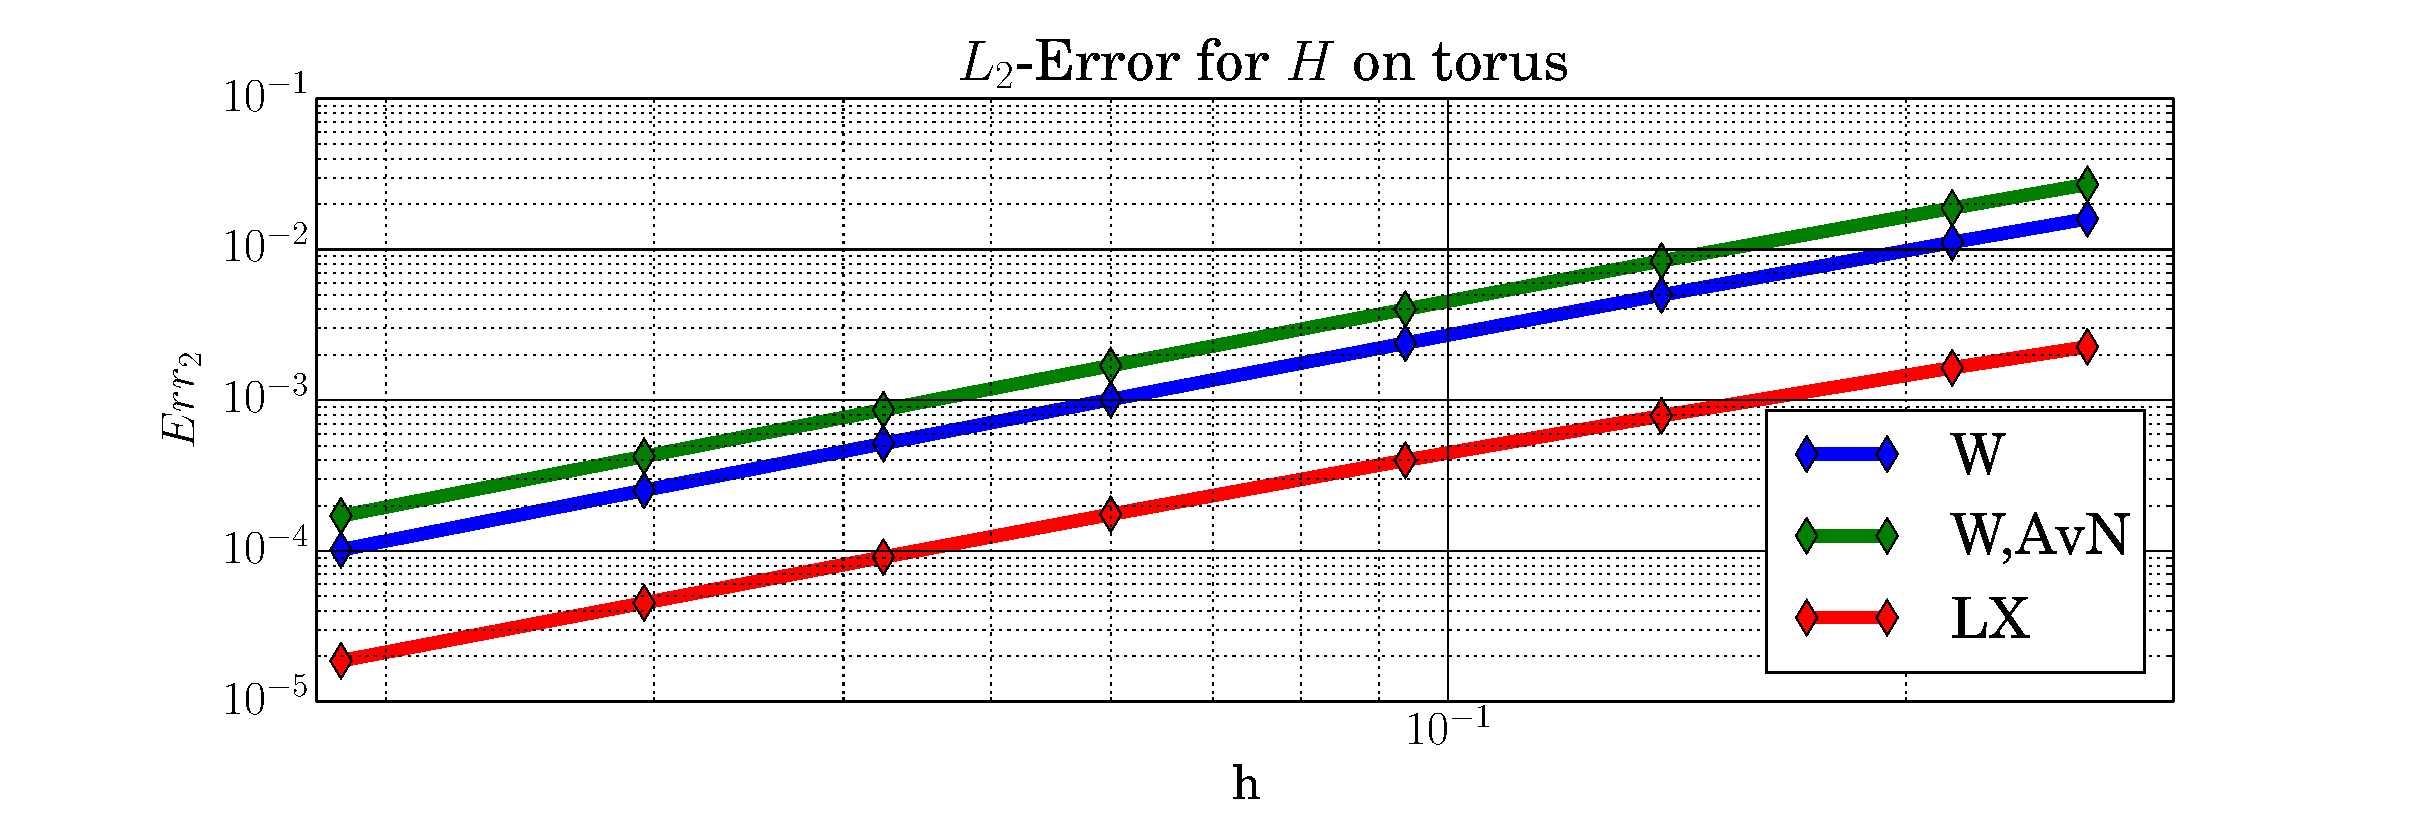
\includegraphics[width=0.99\textwidth]{bilder/torus/L2H.eps}
    \end{minipage}\\
    \begin{minipage}[htp]{.23\textwidth}
      \centering
      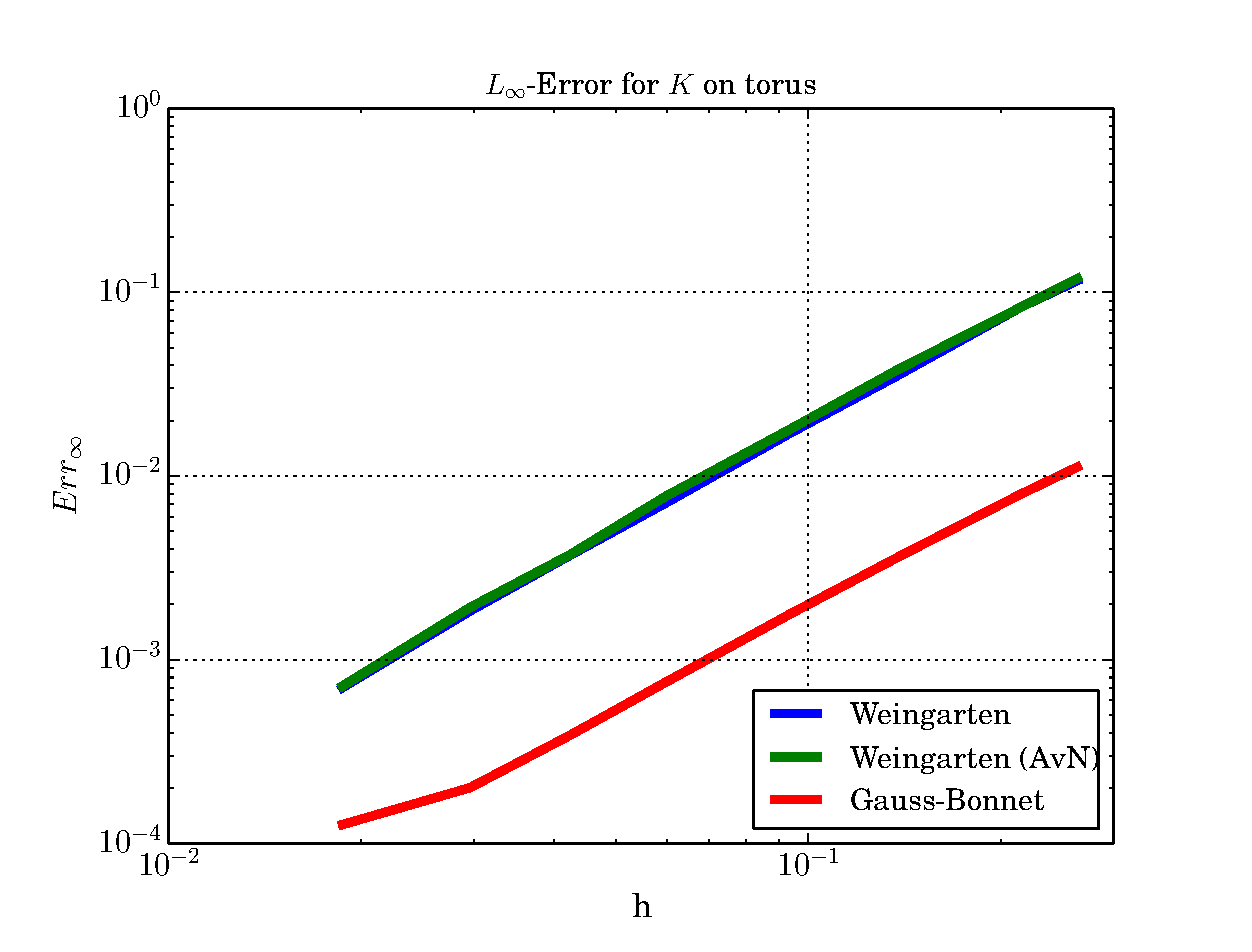
\includegraphics[width=0.99\textwidth]{bilder/torus/LMaxK.eps}
    \end{minipage}\hfill
    \begin{minipage}[htp]{.23\textwidth}
      \centering
      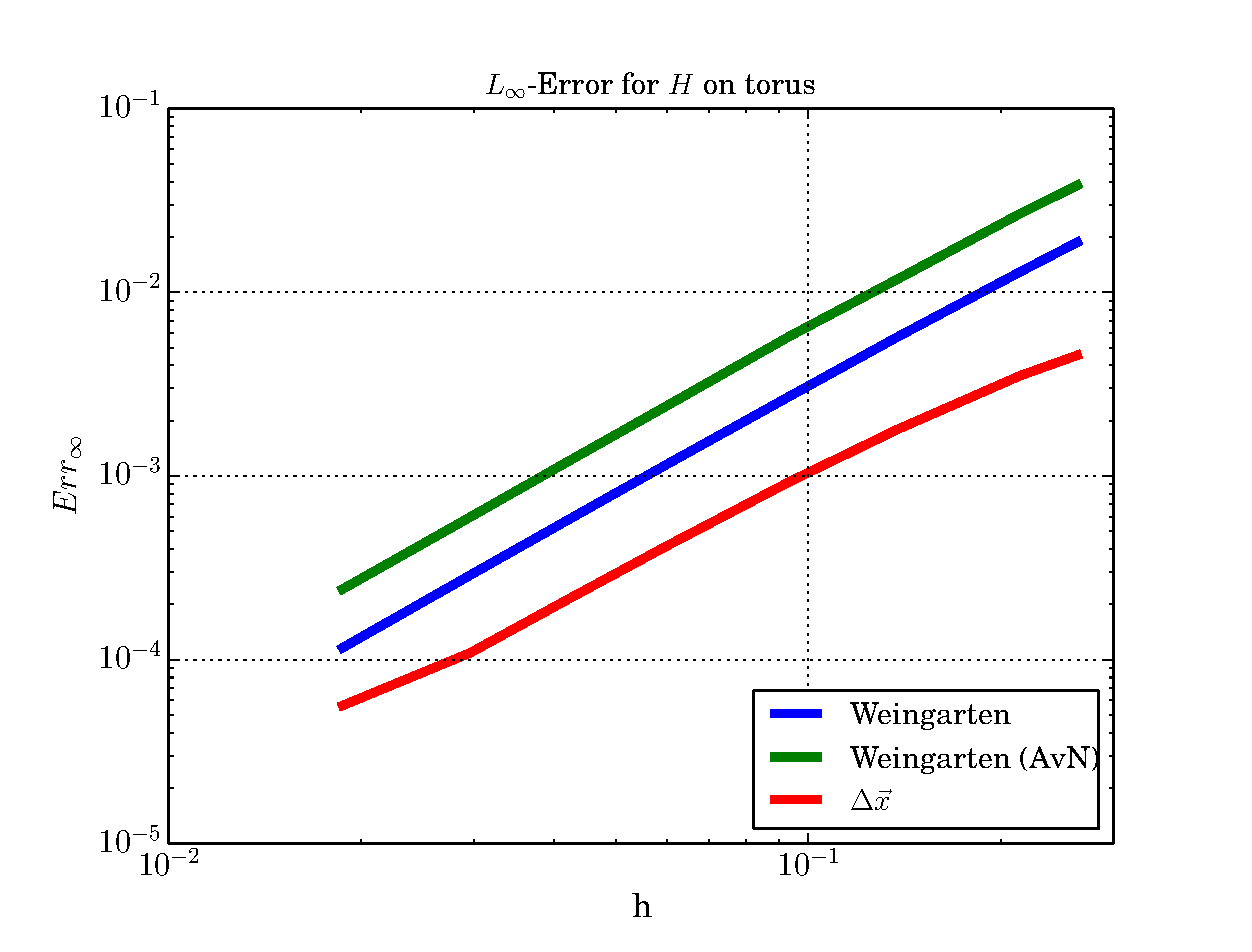
\includegraphics[width=0.99\textwidth]{bilder/torus/LMaxH.eps}
    \end{minipage}
    \caption{Torus: Top row: Gaussian curvature \( K \) (left) and mean curvature \( H \) (right).
                              Middle and bottom row: Relative \( L_{2} \) resp. \( L_{\infty} \) error for \( K \) (left) and
                                                     \( H \) (right) for different \( h \) in a log-log-plot.}
    \label{figTorus}
  \end{figure}



\section*{References}
\bibliography{bibl}
\bibliographystyle{elsarticle-harv}

\end{document}
